% SETTINGS - LATEX
% to change name, title, supervisor etc. go to preamble/preamble.tex
\newcommand{\myFontSize}[0] {12pt}
\newcommand{\mySpacing}[0] {1.5}
\newcommand{\myBibliography}[0] {bib/refs}

\documentclass[\myFontSize,a4paper,twoside,openright,slovak]{book}
\usepackage{titlesec}
\usepackage[utf8]{inputenc}
\usepackage[T1]{fontenc}
\usepackage[slovak]{babel}
\usepackage[a4paper]{geometry}
\usepackage{array}
\usepackage[
    left = \glqq,% 
    right = \grqq,% 
    leftsub = \glq,% 
    rightsub = \grq%
]{dirtytalk}

\usepackage{geometry}
\usepackage{lscape}
\usepackage[parfill]{parskip}
\usepackage{enumitem}
\usepackage{graphicx}
\usepackage{float}
\usepackage{longtable}
\usepackage{setspace}
\usepackage{tabularx}
\usepackage{multirow}
\usepackage{multicol}
\usepackage{fancyhdr}
\usepackage[backend=bibtex,defernums=true]{biblatex}
\usepackage{listing}
\usepackage{lscape}
\usepackage{afterpage}
\usepackage{hyphenat}
\usepackage{lscape}
\usepackage{booktabs}
\usepackage{geometry}
\usepackage{pdfpages}
\usepackage{listings}
\usepackage{needspace}

% SETTINGS - NAMES
\newcommand{\myTitle}[0] {Inteligentný asistent trénovania prezentačných schopností}
\newcommand{\myTitleEN}[0] {Intelligent assistant for training presentation skills}
\newcommand{\myName}[0] {Matej Kandráč}
\newcommand{\mySupervisor}[0] {Ing. Bahleda Miroslav, PhD.}
\newcommand{\myEvidenceNumber}[0] {FIIT-182905-116208}
\newcommand{\myDate}[0] {Máj 2026}
\newcommand{\myDateEng}[0] {May 2026}
\newcommand{\myStudyProgram}[0] {Inteligentné softvérové systémy}
\newcommand{\myStudyProgramEng}[0]{Inteligent software systems}
\newcommand{\myDegreeCourse}[0] {18. Informatika}
\newcommand{\myInstitute}[0] {Ústav informatiky, informačných systémov a softvérového inžinierstva, FIIT STU, Bratislava}


% Spacing
\setstretch{\mySpacing}

\setcounter{secnumdepth}{3}
\setcounter{tocdepth}{3}

\newsavebox\mybox
\pagestyle{plain}
\lhead{\nouppercase{\leftmark}}
\chead{}
\rhead{}
\lfoot{}
\cfoot{\thepage}
\rfoot{}


%style=iso-numeric
%style=authortitle-dw
\defbibheading{references}[Literatúra]{ 
  \chapter*{#1}
  \markboth{#1}{#1}
}
\defbibheading{referencessec}[Literatúra]{ 
  \section*{#1}
  \markboth{#1}{#1}
}
\bibliography{\myBibliography}


% Listing as figure
%\usepackage{libs/minted}
%\usepackage[section]{minted}


% openright does not work :(
\let\tmp\oddsidemargin
\let\oddsidemargin\evensidemargin
\let\evensidemargin\tmp
\reversemarginpar

\titlespacing*{\section}{0pt}{10pt}{5pt}
\titlespacing*{\subsection}{0pt}{8pt}{4pt}
\titlespacing*{\chapter}{0pt}{0pt}{5pt}


\begin{document}

% Minted
% pygmentize -L styles
%\usemintedstyle{autumn}
% Title page
\include{preamble/title}

% Project description
\newpage
\thispagestyle{empty}

\textbf{\large Zadanie práce}

\textbf{Názov zadania}: Inteligentný asistent trénovania prezentačných schopností

\textbf{Názov v angličtine}: Intelligent assistant for training presentation skills

Ústav informatiky, informačných systémov a softvérového inžinierstva, FIIT STU

\textbf{Text zadania}: Z prezentovania pred publikom alebo na verejnosti mávajú hlavne menej skúsení rečníci rôzne obavy, napríklad či bude ich prezentácia dostatočne zaujímavá, zrozumiteľná, plynulá a bez chýb. Tieto obavy sú prirodzené, hlavne pokiaľ nemáme dostatok skúseností, či nie sme zvyknutí verejne vystupovať. Tieto obavy je možné zvládnuť vhodným tréningom.
Oboznámte sa s problematikou úspešného a efektívneho prezentovania a preskúmajte moderné prístupy trénovania prezentačných schopností. Analyzujte najčastejšie problémy, s ktorými sa stretávajú rečníci počas prezentovania, ako sú napríklad nesprávne využívanie neverbálnych a verbálnych prejavov. Identifikujte, ktoré nevhodné javy najviac ovplyvňujú kvalitu prezentácie a zapracujte ich do finálneho riešenia.
Navrhnite inteligentného asistenta na trénovanie prezentačných schopností, ktorý bude použitý pri nácviku verejných prezentácií a bude poskytovať spätnú väzbu na neverbálne a verbálne prejavy rečníka. Využite metódy spracovania obrazu a zvuku na detekciu nevhodných javov počas prezentácie. Na základe zistených javov navrhnite a implementujte systém odporúčaní, ktorý rečníkovi poskytuje spätnú väzbu a usmernenia na zlepšenie jeho prezentačných schopností. Navrhnuté riešenie implementujte a overte.
% 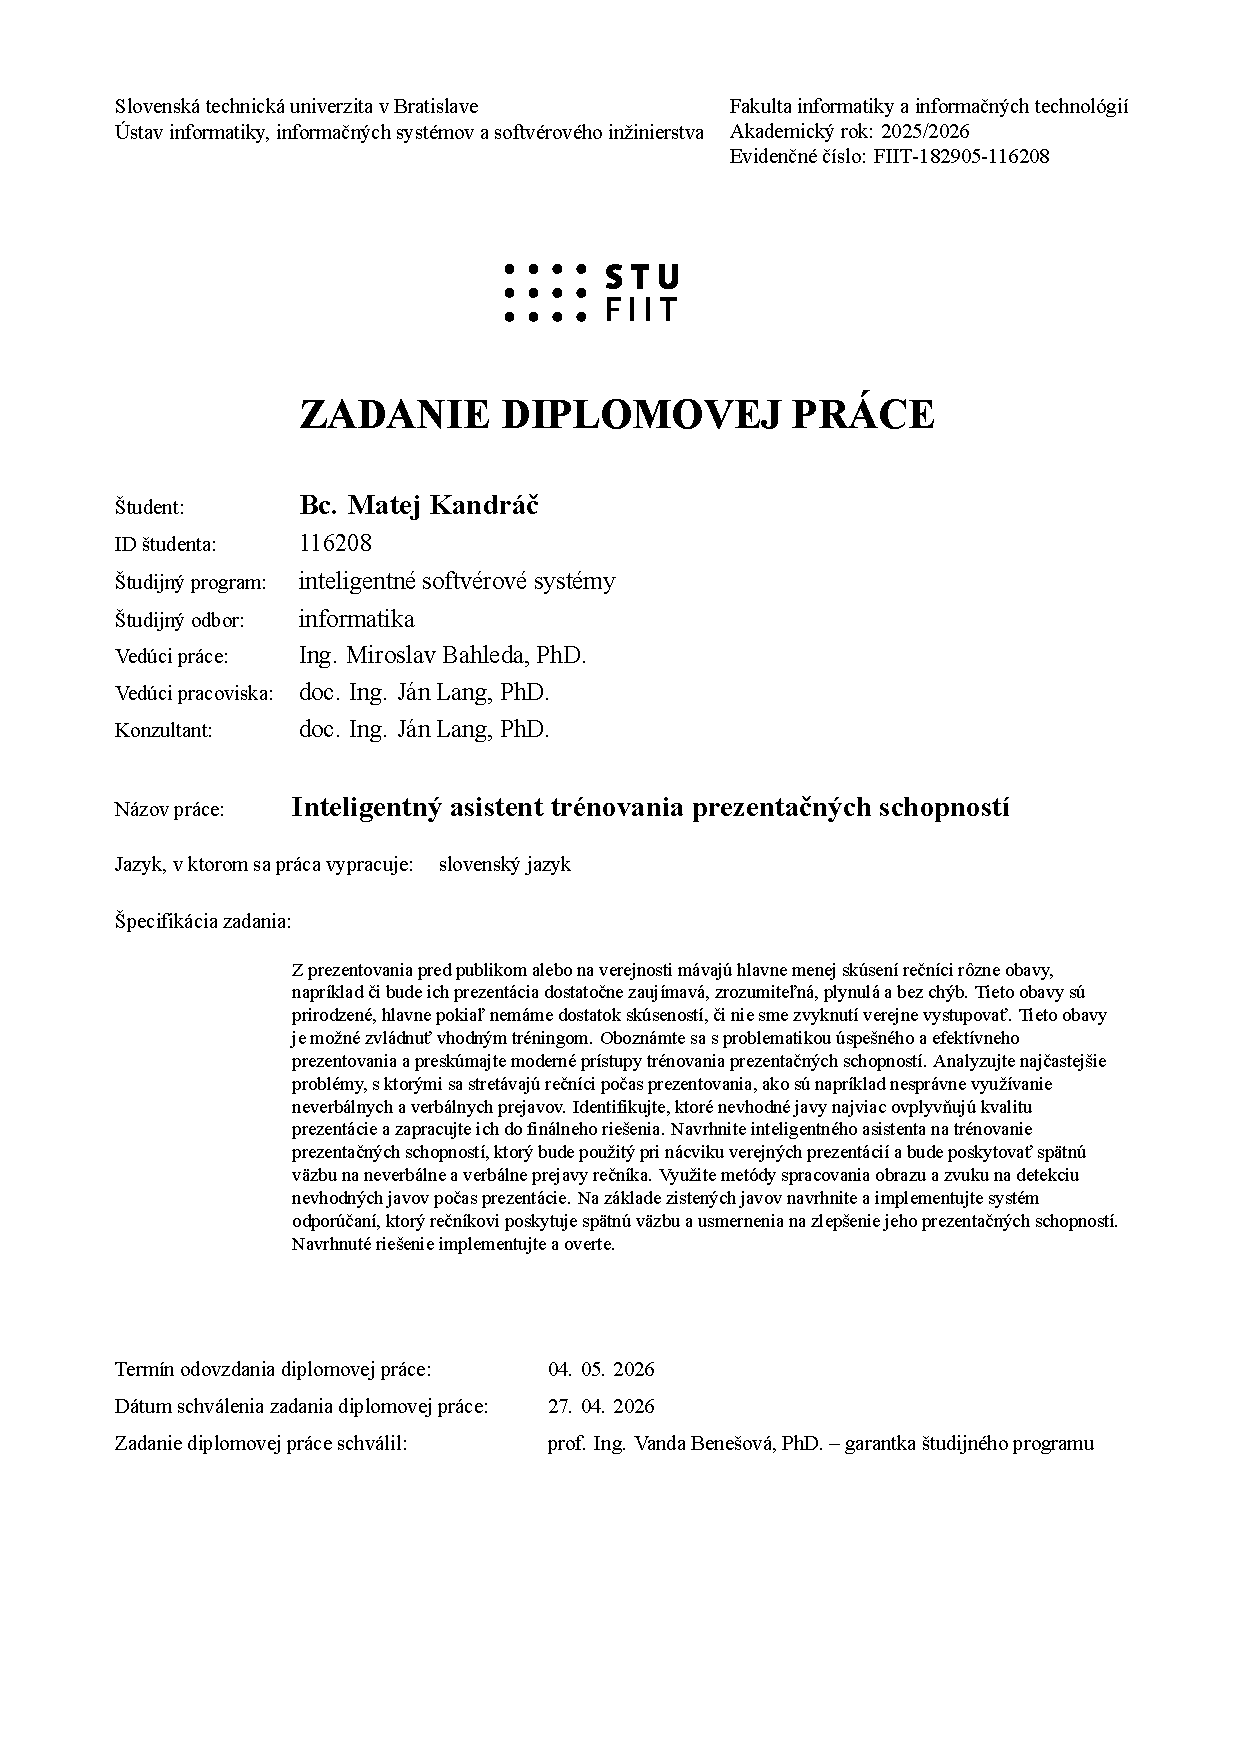
\includepdf[pages=1,scale=0.8]{assets/zadanie.pdf}
\newpage

\thispagestyle{empty}
\mbox{}
\newpage
\thispagestyle{empty}

% Declaration
\include{preamble/declaration}

% Acknowledgements
% \thispagestyle{empty}
\section*{Poďakovanie}

Tu bude podakovanie\ldots

\newpage
\thispagestyle{empty}
\mbox{}
\newpage
\thispagestyle{empty}

% Annotation
\thispagestyle{empty}
\section*{Anotácia}

\begin{minipage}[t]{1\columnwidth}%
Slovenská technická univerzita v Bratislave

FAKULTA INFORMATIKY A INFORMAČNÝCH TECHNOLÓGIÍ
\vskip 5pt
\begin{tabular}{@{}l@{\hspace{10pt}}>{\hyphenrules{nohyphenation}}p{9cm}@{}}

Študijný program: & \myStudyProgram \\

Autor: & \myName \\

Bakalárska práca: & \myTitle \\

Vedúci bakalárskej práce: & \mySupervisor \\
\end{tabular}
\\

\myDate%
\end{minipage}

\bigskip{}
\bigskip{}

\paragraph{}
V tejto diplomovej práci som sa najprv zameral na celú problematiku prezentovania, kde som sa napokon bližšie sústredil na verejné prezentácie. Najprv som sa venoval významu prezentácie ako takej a jej rozdeleniu. Následne som definoval pojem prezentačných schopností a rozdelil komunikáciu na verbálnu a neverbálnu časť. Práca taktiež obsahuje analýzu neverbálnej komunikácie a kladie dôraz na najpodstatnejšie negatívne javy. V práci je zahrnutá aj analýza vlastností hlasu a verbálnej komunikácie. V rámci analýzy je preskúmaná aj problematika časových radov, s dôrazom na segmentáciu a detekciu trendu. Pri porovnaní existujúcich riešení som sa sústredil na tri existujúce riešenia a porovnal som ich. Po analýze som navrhol komplexné riešenie, ktoré využíva mikroslužbovú architektúru pre dosiahnutie flexibilnosti riešenia. Pre používateľov som taktiež navrhol mobilnú aplikáciu pre nahrávanie videí a zobrazenie vizualizácií. Navrhnuté riešenie som napokon úspešne implementoval a otestoval.

\newpage{}
\thispagestyle{empty}

\newpage
\newpage
\thispagestyle{empty}
\mbox{}
\newpage
\thispagestyle{empty}

\section*{Annotation}

\begin{minipage}[t]{1\columnwidth}%
Slovak University of Technology Bratislava 

FACULTY OF INFORMATICS AND INFORMATION TECHNOLOGIES
\vskip 5pt
\begin{tabular}{@{}l@{\hspace{10pt}}>{\hyphenrules{nohyphenation}}p{9cm}@{}}

Degree course: & \myStudyProgramEng \\

Author: & \myName \\

Bachelor's thesis: & \myTitleEN \\

Supervisor: & \mySupervisor \\
\end{tabular}
\\

\myDateEng%
\end{minipage}

\bigskip{}
\bigskip{}

\paragraph{}
In this diploma thesis, I first focused on the overall issue of presenting, eventually narrowing my attention to public presentations. I began by addressing the significance of presentations as such and their classification. I then defined the concept of presentation skills and divided communication into verbal and non-verbal components. The thesis also includes an analysis of non-verbal communication and emphasizes the most significant negative phenomena. It further contains an analysis of voice characteristics and verbal communication. As part of the analysis, the topic of time series is also examined, with a focus on segmentation and trend detection. When comparing existing solutions, I focused on three current approaches and compared them. After the analysis, I proposed a comprehensive solution that uses a microservices architecture to achieve flexibility. I also designed a mobile application for users to record videos and display visualizations. Finally, I successfully implemented and tested the proposed solution.

\newpage
\thispagestyle{empty}
\mbox{}
\newpage

% Table of contents
\tableofcontents
\newpage
\pagestyle{empty}

% List of listings
% \listoffigures\newpage{}
% \renewcommand\listoflistingscaption{List of Listings}
% \listoflistings\newpage{}

% References segment
\begin{refsegment}

\titleformat{\chapter}[display]
{\normalfont\bfseries}{}{0pt}{\Huge}

% Uvod
\clearpage\null
\chapter{Úvod}
\pagestyle{plain}
\pagenumbering{arabic}

Každý z nás počas svojho života aspoň raz prezentoval, či to bola prezentácia jednoduchého školského projektu, pracovný pohovor, obhajoba práce alebo profesionálne vystúpenie pred publikom. Výsledok prezentácie má často významný dopad na našu budúcnosť, alebo na zmýšľanie publika. Schopnosť jasne, presvedčivo a sebavedome komunikovať myšlienky je čoraz dôležitejšia nielen pre manažérov či učiteľov, ale aj pre študentov, výskumníkov či pracovníkov v kreatívnych odvetviach.

Mnohí ľudia však pociťujú pri prezentovaní stres, neistotu alebo nedostatok skúseností, čo im bráni v tom, aby naplno využili svoj potenciál. Tradičné formy nácviku, ako sú školenia, kurzy alebo osobné konzultácie, môžu byť časovo náročné, drahé alebo ťažko dostupné. V tomto kontexte vzniká potreba modernejších a flexibilnejších riešení, ktoré by dokázali poskytnúť individuálnu spätnú väzbu a pomohli používateľom zlepšovať sa.

Jedným z takýchto riešení môže byť inteligentný tréner prezentačných schopností, ktorý by využíval moderné technológie, ako sú umelá inteligencia, analýza reči a analýza obrazu na podporu rozvoja komunikačných zručností. Cieľom tejto práce je priblížiť túto tému a ukázať možnosti, ako môže technológia prispieť k efektívnejšiemu a dostupnejšiemu trénovaniu prezentačných schopností.

% Analyza
\clearpage\null\thispagestyle{empty}
\chapter{Analýza problematiky}
V kontexte prezentácií existuje mnoho foriem prezentovania, ako napríklad pracovné pohovory, verejné vystúpenia alebo aj školské prezentácie. Nakoľko zachytiť všetky tieto formy v rámci jedného riešenia je náročné, rozhodol som sa sústrediť sa na iba verejné prezentácie pred publikom.

Pred samotným návrhom riešenia je potrebné pochopiť základné pojmy spojené s prezentáciami a prezentačnými schopnosťami. V nasledujúcich podkapitolách postupne vysvetlím mnou analyzované pojmy úzko spojené s touto problematikou.

\section{Význam prezentácie}
Cieľom prezentácie je často podať informácie poslucháčom alebo publiku za určitým účelom. Tieto účely sú rôzne a každý zdroj uvádza iné množstvo\cite{purposeOfPresentation}. Základné účely sú:
\begin{itemize}
    \item Informovať
    \item Presvedčiť
    \item Inšpirovať
    \item Pobaviť
\end{itemize}
Pre určenie účelu prezentácie je potrebné si uvedomiť, čo chcem prezentáciou dosiahnúť. Príkladom je napríklad, že idem predniesť nový návrh na reklamnú kampaň pre potenciálneho investora. V tomto prípade chcem presvedčiť moje publikum (investorov), že môj nápad je najlepší. Povedzme že chceme znova predniesť nový návrh na reklamnú kampaň predniesť začiatočníkom v oblasti podnikania. Účel tejto prezentácie by bol inšpiratívny.

Podľa tohto účelu prezentácie vie prezentujúci, na aké informácie alebo formu prejavu sa má najviac sústrediť. Napríklad pri informatívnej prezentácii musí prezentujúci využívať prevažne najpodstatnejšie informácie, pri presviedčaní silné fakty, pri inšpirovaní príbehy alebo inak citové prejavy a pre pobavenie vtipné výroky alebo príbehy\cite{purposeOfPresentation}.

\begin{figure}[H]
    \begin{centering}
        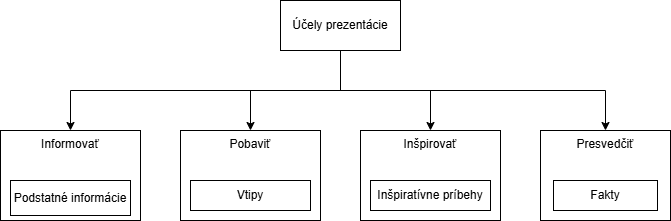
\includegraphics[width=\textwidth]{assets/images/analysis/ucely_prezentacie.png}
        \par\end{centering}
    \caption{Účely prezentácie \label{fig:presentationReasons}}
\end{figure}

\section{Prezentačné schopnosti}
V mojej práci je najpodstatnejšie pochopiť, čo sú to \textbf{prezentačné schopnosti} a čo všetko tento pojem zahŕňa. Prezentačné schopnosti sú vlastnosti a kvality potrebné pre vytváranie a prednášanie presvedčivých prezentácií, ktoré efektívne predávajú informácie a nápady\cite{presentationSkills}. Zahŕňajú nie len hovorené slová ale aj reč tela, vizuálne pomôcky a všeobecnú charizmu prezentujúceho\cite{pressentationSkillsImportance}. Pod vizuálnymi pomôckami si môžeme predstaviť priamo obrazovú prezentáciu, ktorú prezentujúci prednáša.

V mojej práci sa nechcem venovať analýze vizuálnych pomôcok prezentácie, ale sústrediť sa skôr na \textbf{verbálne} a \textbf{neverbálne} aspekty prezentačných schopností, čím docielim zlepšenie samotnej prezentácie. Vizuálne pomôcky sú podstatné pre prezentáciu, no ja sa chcem zamerať na prezentačné schopnosti.

\section{Stavba komunikácie}
Počas mojej analýzy riešenia som narazil na známe pravidlo 7-38-55, ktoré často býva spájané s medziľudskou komunikáciou. Podľa tohto pravidla iba 7 \% významu v komunikácii sprostredkúvajú samotné slová, zatiaľ čo 38 \% pripadá na tón hlasu a až 55 \% na reč tela\cite{73855}. Nakoľko tón hlasu spadá pod neverbálnu komunikáciu, toto pravidlo teda hovorí, že 93\% komunikácie tvorí neverbálna komunikácia.

Hoci je toto pravidlo často citované, v odborných kruhoch býva zároveň aj kritizované. Bolo odvodené z výskumu psychológa Alberta Mehrabiana, ktorý však skúmal veľmi špecifické situácie, predovšetkým rozpory medzi verbálnym a neverbálnym prejavom pri vyjadrovaní emócií. Preto ho nemožno aplikovať univerzálne na všetky formy komunikácie.

Napriek tomu poukazuje na dôležitý fakt, a to že neverbálna zložka komunikácie (napríklad mimika či gestá) má v medziľudskom dorozumievaní výrazný vplyv a neraz môže byť rovnako dôležitá ako samotné slová.

\subsection{Neverbálna komunikácia}
Pod neverbálnou komunikáciou si môžeme predstaviť mnoho vecí. Či už náš postoj, spôsob ako chodíme, výraz tváre, kde máme ruky, no zároveň aj ako rozprávame. V kontexte verejných prezentácií je podstatné nájsť práve také typy neverbálnej komunikácie, ktoré pri nesprávnom vykonávaní nepriaznivo pôsobia na kvalitu prezentácie. Zároveň pri neverbálnej komunikácii je častý problem sebareflexie, pretože tieto prejavy sú často podvedomé, a tým pádom prezentujúci potrebuje dostať spätnú väzbu\cite{intelligentTrainerNguyen}.

Nakoľko negatívne pôsobiacich neverbálnych aspektov je príliž veľa, je potrebné vybrať tie najdôležitejšie. Jeden zo zdrojov vykonal rozhovor s desiatimi expertami v oblasti verejného rozprávania, čo je forma prezentácie, na ktorú som sa rozhodol zamerať\cite{nonverbalImportance}. Po rozhovoroch s odborníkmi zostavili tabľku s údajmi, ktoré rozdelili do viacerých podkategórií.

\begin{figure}[H]
    \begin{centering}
        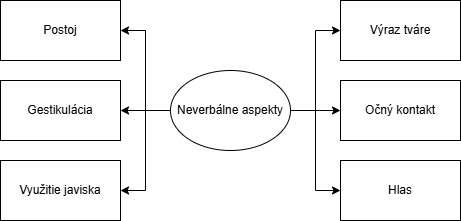
\includegraphics[width=\textwidth]{assets/images/analysis/nonverbals_division.png}
        \par\end{centering}
    \caption{Rozdelenie aspektov neverbálnej komunikácie \label{fig:nonverbalsDivision}}
\end{figure}

Z vyhotovenej tabuľky som vybral tie javy, ktoré najčastejšie spomenuli odborníci a zaradili ich medzi negatívne javy.

\begin{table}[H]
    \centering
    \begin{tabularx}{\textwidth}{|X|X|}
        \hline
        \textbf{Názov javu} & \textbf{Aspekt}  \\
        \hline
        \specialrule{1.2pt}{0pt}{0pt}
        Otočený chrbtom k publiku & Postoj \\ \hline
        Tancovanie (tango a merengue) & Postoj \\ \hline
        Ruky vo vreckach alebo za chrbtom & Postoj \\ \hline
        Žiadna gestikulácia & Gestikulácia \\ \hline
        Držanie / hranie sa s predmetmi & Gestikulácia \\ \hline
        Ruky nad hlavou & Gestikulácia \\ \hline
        "Prázdny" výraz tváre & Výraz tváre \\ \hline
        Žiaden očný kontakt & Očný kontakt \\ \hline
        Státie za počítačom & Využitie javiska \\ \hline
        Konštantný pohyb po javisku & Využitie javiska \\ \hline
        Rozprávanie hlasno pre seba & Hlas \\ \hline
    \end{tabularx}
    \caption{Tabuľka negatívnych javov neverbálnej komunikácie}
    \label{tab:negativeNonverbals}
\end{table}

Jeden z najpodstatnejších aspektov pri verejnom prezentovaní je očný kontakt. Udržiavanie očného kontaktu pomáha pri vytváraní spojenia medzi poslucháčmi, zlepšuje koncentráciu a preukazuje autoritu a sebavedomie\cite{eye_contact}.

Jeden zo zdrojov uvádza, že pri prezentovaní je potrebné využívať signál k zvuku (signal-to-noise). Signál tu definujeme ako akékoľvek pohyby, ktoré dodávajú vášmu rozprávaniu podstatu a ďalej zapájajú publikum, ako napríklad odovzdanie správy rukami alebo očný kontakt s publikom. \cite{nonverbal} Tento pojem znamená, že by prezentujúci mal využívať pohyby spolu s hovoreným slovom. V prípade prepoužívania signálov môže pôsobiť hovorené slovo neprirodzené alebo môžu signály pôsobiť príliš rušivo.

\subsection{Vlastnosti hlasu}
Pri využívani svojho hlasu je potrebné dávať si pozor hneď na niekoľko jeho vlastností. Túto problematiku opisoval v rámci svojej prednášky Julian Treasure\cite{voice} a poukázal na tieto hlasové vlastnosti:
\begin{itemize}
    \item hlasový register
    \item farba hlasu
    \item prozódia
    \item tempo
    \item výška hlasu
    \item hlasitosť
\end{itemize}
Avšak nakoľko detekcia všetkých týchto vlastností hlasu je pomerne komplikovaná, je potrebné z nich vybrať tie najpodstatnejšie. V predošlej sekcii zameranej na neverbálnu komunikáciu odborníci spomenuli niektoré z hore napísaných vlastností hlasu a zároveň aj ako ich negatívne prezentujúci využil. Konkrétne ide o problémy monotónnosti, rýchleho rozprávania a tichého rozprávania.

\subsection{Verbálna komunikácia}
Z hľadiska verbálnej komunikácie sa pri prezentáciach môžeme zamerať na mnoho problémov. S problémami verbalnéj komunikácie je často spôsobená prerušením plynulosti reči, ktorá môže mať viac foriem. Namiesto odprezentovania správne štruktúrovanej reči prezentujúci často hovoria zneistene, opakujú sa a opravújú svoje hovorené slovo.\cite{disfluencies} Častým javom je aj takzvané používanie výplňových slov alebo výplňových zvukov. Niekoľko štúdií preukázalo, že nadmerné používanie výplňových slov alebo zvukov negatívne ovplyvňuje prezentačné zručnosti prezentujúceho.\cite{fillerEffects} \cite{fillerWords} Preto som sa v mojej práci rozhodol venovať sa práve identifikácii týchto slov. V jednom zo zdrojov bolo uvedené, že minimálna prijateľná miera výplňových slov je 1.26 na 100 slov. \cite{fillerWords} Po prekročení tohto limitu začne klesať kredibilita prezentujúceho u poslucháčov.

\section{Časové rady}
Pre pochopenie mojej práce je podstatné pochopiť aj čo sú to časové rady. Časové rady sú jednoducho sekvencie dátových bodov merané v diskrétnych časových bodoch, ktoré sú zoradené chronologicky podľa času\cite{timeSeriesDef}. V mojej práci sa budem zaoberať presne takýmito dátami, nakoľko budem musieť analyzovať jednotlivé vlastnosti hlasu a pohyby používateľa v jednotlivých časových bodoch počas celej prezentácie. Problematika časových radov je pomerne rozsiahlá, no po uvažovaní, ktoré vlastnosti a algoritmy časových radov sa budem sústrediť som sa rozhodol zamerať na dve, a to konkrétne na \textbf{segmentáciu} a \textbf{detekciu trendu}.

\subsection{Segmentácia časových radov}
Segmentácia je rozdeľovanie časových radov na časti, segmenty, ktoré logicky rozdelia dáta\cite{timeSeriesSeg}. Z hľadiska segmentácie je potrebné nájsť také body v časovom rade, ktoré rozdelia dáta podľa odchýlky, priemeru alebo pri zmene trendu. Existuje mnoho algoritmov, ktoré zabezpečujú segmentáciu časových radov. Často sa delia na dve kategórie, a to \textbf{offline} a \textbf{online}. Offline reprezentuje algoritmy, ktoré majú všetky dáta dostupné naraz a online tie, ktoré dáta dostávajú postupne. Ďalšie rozdelenie je podľa spôsobu detekcie bodov zmien, a to sú:
\begin{itemize}
    \item Top-down approach
    \item Bottom-up approach
    \item Sliding window
    \item SWAB (sliding window and bottom-up)
\end{itemize}

Z hľadiska využitia v rámci mojej práce sa môže segmentácia použiť pre rozdelenie dát na úseky, kde ostáva rovnaký trend alebo sa výrazne zmení priemer. Napríklad pri analýze pohybov rúk môže algoritmus rozoznať, že prezentujúci využíva pohyby rúk výrazne v prvej časti prezentácie (trend stúpa alebo je konštantný) a následne ich prestane kvôli tréme využívať (trend klesá). Zároveň body zmien často indikujú anomálie, napríklad prudký pohyb rukami alebo náhle zvýšenie hlasitosti. Tieto údaje môžu byť pre prezentujúceho podstatné, aby si tieto často podvedomé javy uvedomil a zlepšil sa.

\subsection{Detekcia trendu}
Trend je vzor v časovom rade, ktorý sa vyznačuje konzistentným správaním údajov (napríklad stúpajúcim alebo klesajúcim pohybom) v priebehu času\cite{timeSeriesTrend}. V niektorých oblastiach sa trend definuje aj ako všeobecný smer priemeru v dátach\cite{timeSeriesTrendAlgo}.
Pri mojej analýze som narazil na štyri druhy algoritmov na detekciu trendu, ktoré využívajú rozne techniky detekcie, a to:
\begin{itemize}
    \item Fuzzy logic
    \item Štatistické
    \item Regresné
    \item Wavelet
\end{itemize}

Využitie detekcie trendu v rámci mojej práce chcem využiť pri analýze jednotlivých segmentov prezentácie. Napríklad zistím, či v prvom segmente prezentácie prezentujúci prestal postupne využívať gestikuláciu.

\section{Spracovanie audio signálov}

Nakoľko moje riešenie zahŕňa analýzu hlasu a verbálnych aspektov prezentácie, je nevyhnutné pochopiť základné princípy spracovania audio signálov. V tejto sekcii sa zameriam na teoretické základy digitálneho zvuku a metódy jeho spracovania, ktoré sú kľúčové pre implementáciu detekcie vlastností hlasu.

\subsection{Základy digitálneho audio signálu}

Zvuk je vo svojej podstate vlnenie, ktoré sa šíri vzduchom. V analógovej forme je zvuk reprezentovaný ako kontinuálny signál. Na to aby sme vedeli spracovávať zvukové signály musíme analógový signál dostať do digitálnej formy prostredníctvom procesu nazývaného \textbf{vzorkovanie} (sampling)\cite{audioSignalProcessing}.

Digitálny audio signál je teda diskrétna reprezentácia analógového zvukového signálu, kde v pravidelných časových intervaloch meráme amplitúdu (veľkosť) signálu. Výsledkom je časový rad dát, ktoré približne opisujú pôvodný spojitý signál\cite{audioSignalProcessing}. Kvalita tohto odhadu závisí od dvoch základných parametrov: \textbf{vzorkovacej rýchlosti} a \textbf{bitovej hĺbky}. Ak chcem v mojej práci spracovávať zvuk, budem potrebovať signál pripraviť tak, aby bol v čo najlepšej kvalite s ohľadom na ich veľkosť.

\subsection{Vzorkovacia rýchlosť}

Vzorkovacia rýchlosť (sample rate) definuje počet vzoriek (samples) odobratých za sekundu a vyjadruje sa v jednotkách Hertz (Hz). Napríklad vzorkovacia rýchlosť 16 000 Hz znamená, že za jednu sekundu je z analógového signálu odobratých 16 000 diskrétnych vzoriek. Štandardne je vzorkovacia rýchlosť medzi 8kHz a 48kHZ.\cite{sampleRateExplained}

Výber vzorkovacej rýchlosti priamo ovplyvňuje frekvenčné pásmo, ktoré dokáže digitálny signál zachytiť. Podľa \textbf{Nyquistovho-Shannonovho teorému} musí byť vzorkovacia rýchlosť aspoň dvojnásobkom najvyššej frekvencie, ktorú chceme v signáli zachytiť, inak môže nastať aliasing ktorý spôsobí, že sa dáta skreslia a nesprávne sa interpretujú.\cite{nyqshanSamplingTheorem}

V praxi sa využívajú rôzne štandardné vzorkovacie rýchlosti v závislosti od aplikácie:

\begin{itemize}
    \item \textbf{8 kHz} - telefonická kvalita, postačujúca pre rozpoznávanie reči
    \item \textbf{16 kHz} - širokopásmová telefonická kvalita, štandard pre spracovanie reči a rozpoznávanie hlasu
    \item \textbf{22.05 kHz} - nízka kvalita pre multimediálne aplikácie
    \item \textbf{44.1 kHz} - CD kvalita, štandard pre hudbu
    \item \textbf{48 kHz} - profesionálne video a audio produkcie
    \item \textbf{96 kHz a vyššie} - vysokovýkonné audio aplikácie, štúdiové nahrávky
\end{itemize}

Pre analýzu reči sa najčastejšie používa vzorkovacia rýchlosť 16 kHz, pretože ľudský hlas sa väčšinou nachádza vo frekvenčnom pásme do 8 kHz a táto vzorkovacia rýchlosť podľa Nyquistovho teorému postačuje na jeho zachytenie.

\subsection{Bitová hĺbka}

Bitová hĺbka (bit depth) určuje, koľko bitov sa používa na reprezentáciu amplitúdy každej jednotlivej vzorky. Čím vyššia je bitová hĺbka, tým presnejšie dokážeme zachytiť dynamický rozsah signálu\cite{bitDepth}.

Najpoužívanejšie bitové hĺbky sú:

\begin{itemize}
    \item \textbf{8-bit} - 256 úrovní, nízka kvalita, často postačujúca pre jednoduché aplikácie
    \item \textbf{16-bit} - 65 536 úrovní, CD kvalita, štandard pre väčšinu audio aplikácií
    \item \textbf{24-bit} - 16 777 216 úrovní, profesionálne nahrávky
    \item \textbf{32-bit float} - floating-point reprezentácia, používaná pri spracovaní a editácii
\end{itemize}

Dynamický rozsah v decibeloch (dB) možno aproximovať vzťahom:

\begin{equation}
    DR \approx 6.02 \cdot n
\end{equation}

Kde n predstavuje počet bitov. Napríklad 16-bitové audio má dynamický rozsah približne 96 dB, čo je dostatočné pre väčšinu aplikácií spracovania reči. Túto bitovú hĺbku má aj väčšina mobilných telefónov.

\subsection{Normalizácia audio signálov}

Normalizácia je proces úpravy amplitúdy audio signálu tak, aby hodnoty vzoriek spadali do určitého štandardizovaného rozsahu. Tento krok je kritický pri spracovaní audio signálov z rôznych zdrojov, pretože nahrávky môžu mať rôznu hlasitosť a dynamický rozsah.

Existuje niekoľko prístupov k normalizácii, no ja som sa rozhodol použiť normalizáciu \textbf{RMS (Root Mean Square)}.

\textbf{RMS normalization} (Root Mean Square) upravuje signál na základe priemernej energie signálu, čo lepšie odráža vnímanú hlasitosť\cite{rmsNormalization}.

Pri spracovaní audio signálov v digitálnej forme sa často používa normalizácia do rozsahu $[-1, 1]$, čo zodpovedá plnému rozsahu floating-point reprezentácie a minimalizuje riziko orezania signálu (clipping)\cite{floatNormalization}.

\subsection{Extrakcia audio vlastností}

Pre analýzu charakteristík hlasu je potrebné z audio signálu extrahovať relevantné vlastnosti (features). V kontexte analýzy prezentačných schopností sú najpodstatnejšie tieto vlastnosti:

\textbf{Výška hlasu} reprezentuje základnú frekvenciu hlasiviek a je kľúčová pre detekciu monotónnosti. Pre extrakciu pitch existuje niekoľko algoritmov, ako napríklad YIN\cite{yinAlgorithm}, PYIN alebo autokorelačné metódy. Hodnoty pitch pre mužský hlas sa typicky pohybujú v rozsahu 85-180 Hz, pre ženský hlas 165-255 Hz\cite{pitchRange}.

\textbf{Hlasitosť} sa najčastejšie meria pomocou RMS (Root Mean Square) energie signálu v krátkych časových oknách\cite{rmsEnergy}

Tieto extrahované vlastnosti môžu byť následne analyzované ako časové rady, kde môžeme aplikovať metódy segmentácie a detekcie trendov opísané v predchádzajúcich sekciách.

\section{Existujúce riešenia}

V rámci mojej analýzy som sa taktiež rozhodol preskúmať už existujúce riešenia, ktoré sa tejto problematike venovali. Narazil som na niekoľko riešení, no rozhodol som sa vybrať iba niekoľko.

\subsection{MACH}

Mach, alebo My automated conversation coach, je systém, ktorý používa virtuálneho asistenta, ktorý číta výrazy tváre, hlas a prozódiu a ponúka spätnú väzbu v reálnom čase\cite{mach}. Toto riešenie kladie dôraz na použitie virtuálneho asistena, ktorý má pripomínať skutočného trénera, ktorý sa snaží prirodzene reagovať a dávať spätnú väzbu. Po skončení tréningu tento asistent zozbieral a zobrazil niekoľko údajov, a to konkrétne:
\begin{itemize}
    \item Celková dĺžka páuz
    \item Tempo reči (počet slabík za minútu)
    \item "Slabý jazyk" (Výplňové slová, percentuálne vyjadrené pre celkovo hovorené slová)
    \item Variácia výšky hlasu
    \item Úsmev
    \item Kývanie hlavou
    \item Hovorené slová
    \item Hlasitosť
\end{itemize}

\subsection{ROC Speak}

ROC Speak je online platforma poskytujúca spätnú väzbu na úsmev, pohyby tela, moduláciu hlasu a používanie výplňových slov\cite{rocSpeak}. Toto riešenie rozdelilo spätnú väzbu do dvoch komponentov, a to na \textbf{automatizovanú} a \textbf{"subjektívnu"} spätnú väzbu.

Automatizovaná spätná väzba zachytávala niekoľko údajov:
\begin{itemize}
    \item Úsmev
    \item Pohyby tela
    \item Hlasitosť a výška hlasu
    \item Tanskript a prozódia slov
    \item "Slabé slová"
\end{itemize}

Subjektívna spätná väzba bola vykonávaná formou komentárov a hodnotenia od iných ľudí. Systém dokonca automaticky ohodnocoval, či je daný komentár negatívny alebo pozitívny a následne zobrazoval najrelevantnejšie komentáre používateľovi.

\subsection{GestureLens}

GestureLens je systém vizuálnej analýzy, ktorý uľahčuje preskúmanie používania gest vo videách z prezentácií, a to na základe gest aj obsahu\cite{gestureLens}. Snaží sa nájsť podobnosti gést ktoré spája s hovoreným slovo ma využíva dynamic time warping pre zisťovanie podobností gest.

Toto riešenie dokáže detekovať a analyzovať:
\begin{itemize}
    \item Pohyby rúk
    \item Korelácie hovoreného slova s gestami
    \item Transkripcia hovoreného slova
    \item Priesorové využitie gest (heatmapa)
\end{itemize}

Tento systém je pomerne komplikovaný a detailne analyzuje primárne pohyby rúk.

\subsection{Porovnanie riešení}

Po analýze týchto troch existujúcich riešení som sa rozhodol vytvoriť tabuľku parametrov, ktorá zachytáva podstatné parametre jednotlivých riešení, ako aj to, či detekujú negatívne javy, ktoré som opísal ako najpodstatnejšie v časti neverbálnej a verbálnej komunikácii.

\begin{table}[H]
    \centering
    \begin{tabularx}{\textwidth}{|X|X|X|X|}
        \hline
        & \textbf{MACH} & \textbf{ROC Speak} & \textbf{GestureLens} \\
        \hline
        \specialrule{1.2pt}{0pt}{0pt}
        Platforma & Desktop & Web & Web \\
        \hline
        Otočenie chrbtom k publiku & Nie & Nie & Nie \\
        \hline
        Tancovanie & Nie & Nie & Nie \\
        \hline
        Ruky vo vreckách & Nie & Nie & Nie \\
        \hline
        Žiadna gestikulácia & Áno & Áno & Áno \\
        \hline
        Držanie / hranie sa s predmetmi & Nie & Nie & Nie \\
        \hline
        Ruky nad hlavou & Nie & Nie & Áno \\
        \hline
        Nedostatočná mimika & Áno & Áno & Nie \\
        \hline
        Očný kontakt & Áno & Nie & Nie \\
        \hline
        Státie za počítačom & Nie & Nie & Nie \\
        \hline
        Konštantný pohyb po javisku & Áno & Áno & Áno \\
        \hline
        Rozprávanie hlasno pre seba & Nie & Nie & Nie \\
        \hline
        Výplňové slová & Áno & Áno & Nie \\
        \hline
        Monotónnosť & Áno & Áno & Nie \\
        \hline
        Vysoké tempo reči & Áno & Áno & Nie \\
        \hline
        Nedostatočná hlasitosť & Áno & Áno & Nie \\
        \hline
        Hlavné zameranie & Mimika, očný kontakt, gestikulácia, tempo reči a výplňové slová & Intenzita úsmevu, pohyby tela a verbálne aspekty & Korelácia hovoreného slova s gestikuláciou \\
        \hline
    \end{tabularx}
    \caption{Tabuľka porovnania atribútov riešení}
    \label{tab:attributesTable}
\end{table}

Z tejto tabuľky môžeme vidieť, že žiadne z aplikácií nesledujú problémy spojené s postojom prezentujúceho, ako tancovanie, ruky vo vreckách alebo hranie sa s predmetmi.

\section{Definícia problému}

Na základe analýzy existujúcich riešení a preštudovanej literatúry som identifikoval niekoľko kľúčových medzier, ktoré poukazujú na potrebu komplexnejšieho prístupu k trénovaniu prezentačných schopností.

\subsection{Fragmentácia existujúcich riešení}

Ako je vidieť z tabuľky porovnania riešení (tabuľka \ref{tab:attributesTable}), \textbf{neexistuje jednotné riešenie}, ktoré by komplexne pokrývalo všetky podstatné aspekty prezentačných schopností. Analyzované systémy sa zameriavajú selektívne na konkrétne oblasti:

\begin{itemize}
    \item \textbf{MACH} sa primárne sústreďuje na mimiku, očný kontakt a verbálne aspekty (tempo reči, výplňové slová), no zanedbáva detailnú analýzu pohybov tela a postoja
    \item \textbf{ROC Speak} kladie dôraz na intenzitu úsmevu a verbálne aspekty, avšak neanalyzuje očný kontakt ani špecifické negatívne javy spojené s postojom
    \item \textbf{GestureLens} sa detailne venuje korelácii gest s hovoreným slovom, no úplne opomína analýzu verbálnych aspektov ako monotónnosť či výplňové slová
\end{itemize}

Žiadne z týchto riešení nepokrýva komplexne \textbf{verbálnu aj neverbálnu komunikáciu} súčasne. Konkrétne, neexistuje riešenie, ktoré by analyzovalo:

\begin{enumerate}
    \item \textbf{Neverbálne aspekty}: postoj (tancovanie, ruky vo vreckách), detailné pohyby rúk, očný kontakt, mimiku
    \item \textbf{Vlastnosti hlasu}: monotónnosť, hlasitosť, výška tónu, tempo reči
    \item \textbf{Verbálne aspekty}: výplňové slová, plynulosť reči
\end{enumerate}

v rámci jedného integrovaného systému.

\subsection{Technologické obmedzenia}

Ďalším zásadným problémom je, že analyzované riešenia neposkytujú prístup k \textbf{surových dátam} získaných počas analýzy. Systémy ako MACH či ROC Speak fungujú ako uzavreté riešenia (black-box), ktoré prezentujú iba finálne výsledky používateľovi. Neposkytujú možnosť:

\begin{itemize}
    \item Exportu časových radov pohybov tela (landmarks)
    \item Prístupu k extrahovaným vlastnostiam hlasu (pitch, RMS energia)
    \item Vlastného spracovania a analýzy týchto dát
    \item Implementácie pokročilých metód analýzy časových radov (segmentácia, detekcia zmien trendu)
\end{itemize}

Táto skutočnosť vytvára potrebu \textbf{vlastného riešenia pre extrakciu a spracovanie dát}, ktoré umožní nielen detekciu negatívnych javov, ale aj ich hlbšiu analýzu prostredníctvom metód spracovania časových radov.

\subsection{Nedostatok komplexnej analýzy časových radov}

Analyzované riešenia poskytujú prevažne \textbf{agregované štatistiky} (napríklad celkový počet výplňových slov, priemerná hlasitosť), no chýba im časová dimenzía analýzy. Prezentujúcemu nepovedia:

\begin{itemize}
    \item V ktorom momente prezentácie prestali využívať gestikuláciu
    \item Kedy sa zmenilo ich tempo reči alebo monotónnosť
    \item Kde nastali kritické body zmien v ich správaní
    \item Ako sa vyvíjali jednotlivé vlastnosti počas celej prezentácie
\end{itemize}

Práve \textbf{identifikácia kritických bodov zmien} a analýza trendov v časových radoch môže prezentujúcemu poskytnúť oveľa hodnotnejšiu spätnú väzbu než len celkové čísla.

\subsection{Formulácia problému}

\textbf{Problémom je absencia komplexného systému pre trénovanie prezentačných schopností, ktorý by:}

\begin{enumerate}
    \item Integroval analýzu verbálnych, neverbálnych aspektov aj vlastností hlasu v jednom riešení
    \item Umožnil extrakciu a spracovanie surových dát (landmarks tela, audio features) pre vlastnú analýzu
    \item Využíval metódy analýzy časových radov (segmentáciu, detekciu trendov) na identifikáciu kritických bodov zmien
    \item Poskytoval detailnú časovú analýzu, nie len agregované štatistiky
    \item Bol dostupný širokej verejnosti prostredníctvom mobilných zariadení
\end{enumerate}

\textbf{Prečo je tento problém dôležitý?} Prezentačné schopnosti sú kľúčové v mnohých oblastiach života - od akademického prostredia cez pracovné pohovory až po profesionálne vystúpenia. Tradičné formy nácviku (kurzy, tréningy) sú časovo aj finančne náročné a nie vždy dostupné. Moderný systém, ktorý poskytne komplexnú spätnú väzbu využitím pokročilých metód spracovania videa a zvuku, môže demokratizovať prístup k trénovaniu prezentačných schopností a umožniť používateľom efektívne sa zlepšovať aj bez prítomnosti fyzického trénera.

Moje riešenie sa preto zameriava na vytvorenie takéhoto komplexného systému, ktorý eliminuje uvedené medzery existujúcich riešení.

% Navrh
\clearpage\null\thispagestyle{empty}
\chapter{Návrh  riešenia}

Mojim návrhom je implementácia systému, ktorá umožní používateľovi prípravu pred prezentáciou a taktiež aj spracovanie už existujúceho záznamu prezentácie. Rozhodol som sa využiť \textbf{mobilné zariadenia}, ktoré dnes má takmer každý človek a sú vybavené vstavanou kamerou. Z týchto zariadení vytvorí používateľ video, ktoré následne odošle pomocou mobilnej aplikácie na aplikačný server, ktorý prezentáciu zanalyzuje a poskytne spätnú väzbu. Moja aplikácia teda bude fungovať na \textbf{záznamoch} a nie na živom prenose. Aplikácie bude ponúkať dve základné funkcie a to:
\begin{itemize}
    \item Trénovanie konkrétneho javu
    \item Celková analýza prezentácie
\end{itemize}
Pri \textbf{trénovaní konkrétneho javu} si používateľ zvolí jednu z možností, na čo sa chce zamerať a následne natočí video, ktoré mu systém následne zhodnotí. Príkladom je, že používateľ sa chce naučiť správne využívať očný kontakt, tak moje riešenie mu dovolí umiestniť zariadenie dostatočne ďaleko a následne natočiť video a odoslať pre spracovanie. V tomto móde systém spúšta iba jeden druh detekcie a sústredí sa naň.

\textbf{Celková analýza prezentácie} poskytuje spätnú väzbu vo všetkých oblastiach prezentácie. V prípade, že systém nevie spoľahlivo určiť niektorú z funkcií, oznámi to používateľovi a tento jav nedetekuje. Napríklad ak nevie kamera zachytiť zápästia používateľa z dôvodu, že je ho ruky su mimo kameru, upozorní ho na to.

\section{Špecifikácia požiadaviek}
Pred samotnou implementáciou som definoval niekoľko funkčných požiadaviek, ktoré by aplikácia mala spĺňať. Pri rozhodovaní, ktoré údaje budem detekovať som sa odrážal od môjho výskumua porovnaní existujúcich riešení, ktorý bol bližšie popísaný v sekcii analýza problematiky.
\begin{itemize}
    \item \textbf{Detekcia očného kontaktu}: Systém musí vedieť rozpoznať, či sa prezentujúci pozerá smerom do publika a nie je k nemu otočený chrbtom. Pre detekciu tohto javu sa využije viditeľnosť očí voči kamere, ktorá bude pred prezentujúcim.
    \item \textbf{Detekcia pohybu bokov}: Systém musí vedieť detekovať negatívny jav, nazývaný ako tancovanie (pohyb bokov zo strany na stranu). Detekcia bude počítaná akceleráciou stredu medzi bokmi, a bude detekovať kývanie z prava do ľava a z predu do zadu.
    \item \textbf{Detekcia pohybov rúk}: Systém musí vedieť detekovať nedostatočné pohyby rúk v prezentácii. Taktiež počítaná sledovaním akcelerácie rúk. Zároveň bude systém sledovať opakujúce sa gestá.
    \item \textbf{Detekcia monotónnosti}: Systém musí vedieť detekovať monotónny hlas. Monotónnosť hlasu je definovaná ako konštantný tón hlasu počas prezentácie. Bude sa teda sledovať zmena tónu hlasu.
    \item \textbf{Detekcia hlasitosti}: Systém musí vedieť detekovať nízku hlasitosť prezentujúceho.
    \item \textbf{Detekcia výplňových slov}: Systém musí vedieť detekovať výplňové slová.
    \item \textbf{Detekcia kritických bodov zmien}: Systém musí pre relevantné kritériá uvedené vyššie definovať kritické body, kedy sa drasticky zmenil doterajší priebeh. Ide napríklad o definovanie hranice, kedy prezentujúci prestal náhle využívať všetky pohyby rúk, alebo že v prvej minúte prezentácie využíval veľké množstvo výplňových slov.
\end{itemize}

\newpage

\section{Architektúra riešenia}
Nakoľko som počas analýzy zistil, že nevhodných javov ktoré je možné detekovať je veľke množstvo, navrhujem mikroslužbovou architektúru, kde každá mikroslužba bude detekovať skupinu súvisiacich negatívnych javov. Dôvodom použitia mikroslužieb je ich vlastnosť jednoduchého nasadzovania, ktorá môže byť využitá pri pridávaní nových detekcií. Zároveň mikroslužbová architektúra umožnuje technologickú voľnosť, ktorá by sa v prípade rozširovania mojej práce zišla. Všeobecná architektúra by obsahovala:
\begin{itemize}
    \item Mobilnú aplikáciu
    \item API Gateway
    \item Mikroslužba pre analýzu videa
    \item Mikroslužby pre detekciu javov
    \item Databáza
\end{itemize}


Pre pochopenie som vytvoril sekvenčný diagram, ktorý znázorňuje interakciu používateľa so systémom, kde chce detekovať konkrétne pohyb rúk.

\begin{figure}[H]
\begin{centering}
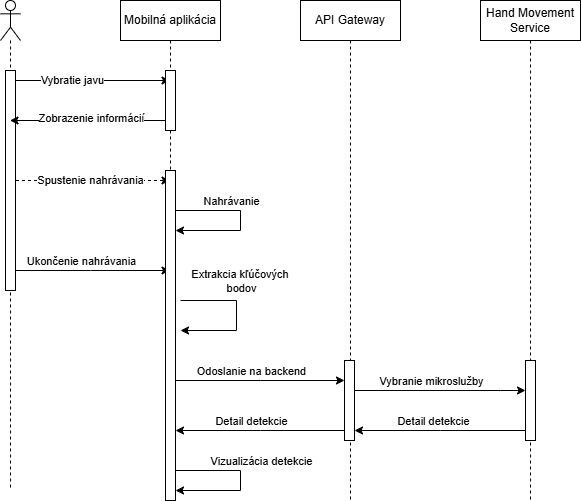
\includegraphics[width=\textwidth, height=12cm]{assets/images/implementation/detekciaKonkretne.png}
\par\end{centering}
\caption{Príklad interakcie s aplikáciou v móde trénovania konkrétneho javu \label{fig:sequenceSingleDetect}}
\end{figure}

Pri detekcii všetkých negatívnych javov pribúda ešte mediator, ktorý po nahratí videa spustí detekciu na všetkých mikroslužbách a vytvorí komplexnú odpoveď so všetkými údajmi.

\begin{figure}[H]
\begin{centering}
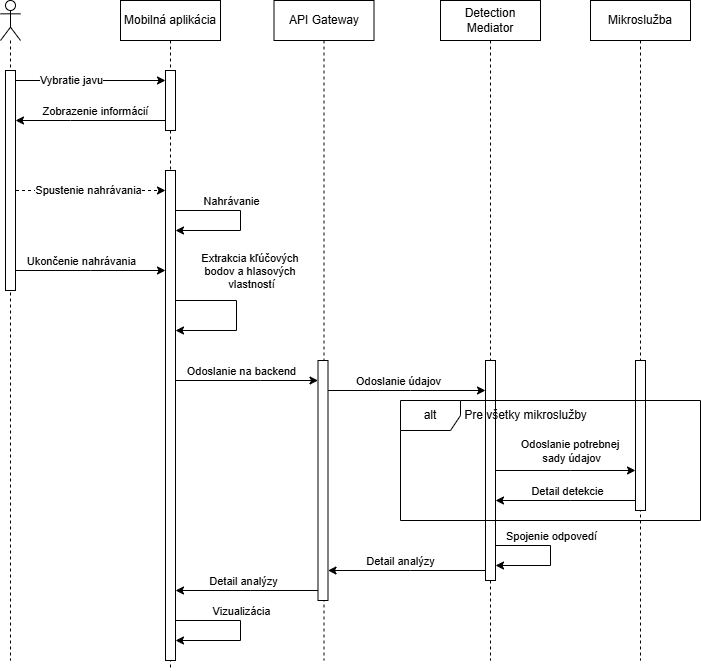
\includegraphics[width=\textwidth]{assets/images/implementation/detectionAll.png}
\par\end{centering}
\caption{Príklad interakcie s aplikáciou v móde celkovej analýzy\label{fig:sequenceAllDetect}}
\end{figure}

\newpage
Celkový diagram systému bude teda nasledovný:

\begin{figure}[H]
\begin{centering}
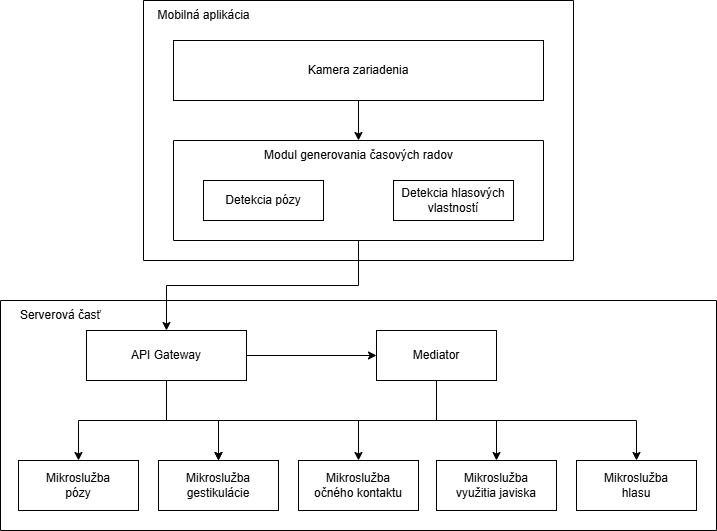
\includegraphics[width=\textwidth]{assets/images/implementation/architecture.png}
\par\end{centering}
\caption{Architektúra aplikácie \label{fig:sequenceAllDetect}}
\end{figure}

Diatram je rozdelený na mobilnú aplikáciu a serverovú časť.

\textbf{Mobilná aplikácia} má za úlohu vytvorenie videa a vytvorenie časových radov pre video. Tieto údaje následne posielá na \textbf{API Gateway}, ktorý slúži ako proxy, ktoré posunie iba podstatné údaje do \textbf{mikroslužby}, ktorá detekuje potrebné vlastnosti. Taktiež je zobrazený aj \textbf{mediator}, ktorý sa bude využívať pri detekcii všetkých javov.

\subsection{Použité technológie}

Z hľadiska využitých technológií chcem pre mobilnú aplikáciu využiť framework \textbf{Flutter}, čim zabezpečím dostupnosť aplikácie pre hlavné platformy na mobilných zariadeniach. Pre serverovú časť chcem použiť framework \textbf{django}, ktorý je využíva programovací jazyk Python. Tento jazyk je štandardným jazykom pre strojové učenie a disponuje veľkým množstvom knižníc pre analýzu časových radov. Pre detekciu kľúčových bodov polohy využijem \textbf{Google ML Kit} a konkrétne \textbf{pose detection}, ktorá mi poskytne všetky potrebné kľúčové body. Nasledujúci obrázok zobrazuje všetky body, ktoré táto knižnica vie detekovať\cite{googleMLKit}.

\begin{figure}[H]
\begin{centering}
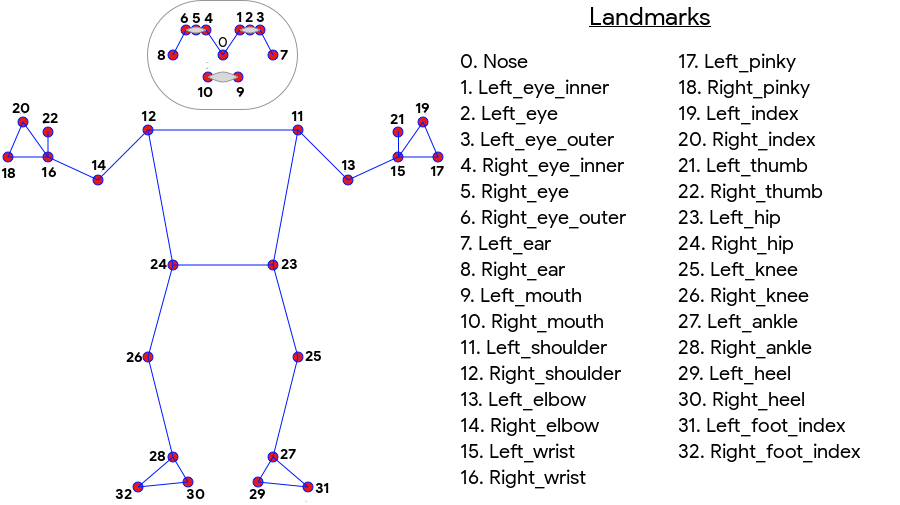
\includegraphics[width=\textwidth]{assets/images/implementation/poseDetecion.png}
\par\end{centering}
\caption{Kľúčové body detekované Google ML kitom \label{fig:sequenceAllDetect}}
\end{figure}

% Implementacia
\clearpage\null\thispagestyle{empty}
\chapter{Implementácia riešenia}

V tejto kapitole podrobne popisujem implementáciu navrhnutého systému, kľúčové algoritmy, dátové štruktúry a technické riešenia použité pri realizácii jednotlivých komponentov.

\section{Prehľad implementovanej funkcionality}

V rámci doterajšej práce som implementoval nasledujúce komponenty systému:

\begin{itemize}
    \item \textbf{API Gateway} (Spring Boot/Kotlin) - vstupný bod systému, správa HTTP requestov a multipart file upload
    \item \textbf{Video Analysis Service} - extrakcia landmarks pomocou MediaPipe Pose
    \item \textbf{Audio Analysis Service} - extrakcia zvukovej stopy a audio vlastností
    \item \textbf{Eye Contact Analysis Service} - detekcia očného kontaktu a looking away events
    \item \textbf{Arm Movement Analysis Service} - detekcia pohybov rúk a gestikulácie
    \item \textbf{Hip Movement Analysis Service} - detekcia negatívneho javu "tancovanie"
    \item \textbf{Pitch Analysis Service} - analýza monotónnosti hlasu
    \item \textbf{Volume Analysis Service} - analýza hlasitosti reči
    \item \textbf{Filler Words Analysis Service} - detekcia výplňových slov pomocou Whisper
\end{itemize}

Všetky mikroslužby sú kontajnerizované pomocou Docker a komunikujú prostredníctvom REST API. Dáta sú ukladané do centrálnej PostgreSQL databázy.

\section{Spracovanie videa}

\subsection{Extrakcia kľúčových bodov pomocou MediaPipe}

Pre detekciu polohy tela v každom snímku videa využívam knižnicu \textbf{MediaPipe Pose} od spoločnosti Google. MediaPipe je schopný v real-time detekovať 33 kľúčových bodov (landmarks) ľudského tela bez potreby špeciálneho hardvéru.

\subsubsection{Použité landmarks}

MediaPipe Pose poskytuje nasledujúce kľúčové body relevantné pre moju analýzu:

\begin{itemize}
    \item \textbf{Tvár}: nos (0), ľavé oko (2), pravé oko (5), ľavé ucho (7), pravé ucho (8)
    \item \textbf{Trup}: ľavé rameno (11), pravé rameno (12), ľavý bok (23), pravý bok (24)
    \item \textbf{Ruky}: ľavý lakeť (13), pravý lakeť (14), ľavé zápästie (15), pravé zápästie (16)
\end{itemize}

Každý landmark obsahuje:
\begin{itemize}
    \item \textbf{x, y, z súradnice} - normalizované pozície v 3D priestore
    \item \textbf{visibility} - confidence score (0-1) indikujúci viditeľnosť bodu
\end{itemize}

% TODO: Placeholder pre obrázok MediaPipe landmarks
% \begin{figure}[H]
% \centering
% \includegraphics[width=0.8\textwidth]{assets/images/implementation/mediapipe_landmarks_example.png}
% \caption{Príklad detekcie MediaPipe Pose landmarks na testovom videu}
% \label{fig:mediapipe_landmarks}
% \end{figure}

\subsubsection{Postup extrakcie}

Extrakcia landmarks prebieha v nasledujúcich krokoch:

\begin{enumerate}
    \item Video súbor je načítaný pomocou OpenCV (\texttt{cv2.VideoCapture})
    \item Pre každý snímok (frame) sa vykoná:
    \begin{itemize}
        \item Konverzia z BGR do RGB farebného priestoru
        \item Spustenie MediaPipe Pose detekcie
        \item Extrakcia 33 landmarks s ich súradnicami a visibility
        \item Uloženie landmarks do dátovej štruktúry s timestamp
    \end{itemize}
    \item Landmarks sú uložené do databázy spolu s frame\_index a timestamp
\end{enumerate}

\subsubsection{Dátová štruktúra}

Landmarks sú ukladané v PostgreSQL databáze v nasledujúcej štruktúre:

\begin{verbatim}
landmark (
    id SERIAL PRIMARY KEY,
    frame_data_id INTEGER REFERENCES frame_data(id),
    type VARCHAR(50),     -- napr. "nose", "left_wrist"
    x DECIMAL(10,6),      -- normalizovaná súradnica 0-1
    y DECIMAL(10,6),
    z DECIMAL(10,6),
    visibility DECIMAL(5,4)  -- confidence 0-1
)
\end{verbatim}

Táto štruktúra umožňuje efektívne dopyty pre jednotlivé mikroslužby, ktoré si načítavajú len potrebné landmarks (napr. Eye Contact Analysis potrebuje len landmarks očí a tváre).

\section{Spracovanie zvuku}

\subsection{Extrakcia zvukovej stopy}

Audio stopa je extrahovaná z nahratého videa pomocou nástroja \textbf{ffmpeg} ihneď po uploade videa. Výsledný audio súbor je uložený vo formáte WAV s nasledujúcimi parametrami:

\begin{itemize}
    \item \textbf{Formát}: WAV (PCM)
    \item \textbf{Vzorkovacia frekvencia}: 16 kHz
    \item \textbf{Kanály}: mono (1 kanál)
    \item \textbf{Bitová hĺbka}: 16-bit
\end{itemize}

Príkaz ffmpeg pre extrakciu:
\begin{verbatim}
ffmpeg -i video.mp4 -vn -acodec pcm_s16le -ar 16000 -ac 1 audio.wav
\end{verbatim}

\subsection{Normalizácia}

Audio signál je normalizovaný na škálu od -1 do 1. Týmto zabezpečím, aby boli dáta v rovnakej škále nezávisle od nahrávaného zariadenia. Normalizácia je implementovaná pomocou knižnice librosa:

\begin{verbatim}
audio_data = librosa.util.normalize(audio_data)
\end{verbatim}

Toto je dôležité najmä pre budúce rozšírenia systému, kde by sa mohli audio dáta využiť pre trénovanie modelov strojového učenia.

\subsection{Vzorkovacia rýchlosť}

Vzorkovacia rýchlosť (sample rate) reprezentuje počet meraných vzoriek za sekundu. Rôzne nahrávače zariadenia môžu mať rozdielnu vzorkovaciu frekvenciu (44.1 kHz, 48 kHz, atď.).

Pre zabezpečenie konzistencie analýzy vykonávam resampling všetkých audio súborov na fixnú frekvenciu \textbf{16 kHz}. Túto hodnotu som zvolil na základe priemyselných štandardov pre speech processing\cite{sampleRate}. Resampling je implementovaný pomocou librosa:

\begin{verbatim}
audio_data = librosa.resample(audio_data, orig_sr=orig_sr, target_sr=16000)
\end{verbatim}

Dôvod normalizácie vzorkovacej rýchlosti je ten, že moje algoritmy pracujú s počtom frame-ov. Napríklad ak detekujem monotónnosť ako "pitch sa nezmenil na 10 za sebou idúcich frame-och", rozdielna vzorkovacia rýchlosť by znamenala rozdielny časový úsek.

\subsection{Bitová hĺbka}

Bitová hĺbka definuje presnosť merania amplitúdy zvukového signálu. Používam \textbf{16-bit PCM}, čo poskytuje dostatočnú presnosť pre analýzu reči (96 dB dynamický rozsah) pri rozumnej veľkosti súboru. Pre porovnanie, 8-bit by poskytoval len 48 dB dynamický rozsah, čo by bolo nedostatočné pre detekciu jemných zmien v hlasitosti.

\subsection{Extrakcia audio vlastností}

Pre analýzu vlastností hlasu využívam knižnicu \textbf{librosa}, ktorá poskytuje funkcie pre extrakciu pitch a hlasitosti.

\subsubsection{Pitch (výška tónu)}

Pitch reprezentuje základnú frekvenciu hlasu (F0). Pre extrakciu pitch využívam \textbf{YIN algoritmus}, ktorý je robust voči šumu a poskytuje presné výsledky pre ľudský hlas:

\begin{verbatim}
pitches = librosa.yin(
    audio_data,
    fmin=librosa.note_to_hz('C2'),  # 65 Hz
    fmax=librosa.note_to_hz('C7')   # 2093 Hz
)
\end{verbatim}

Rozsah 65-2093 Hz pokrýva celý rozsah ľudského hlasu (mužský hlas ~85-180 Hz, ženský hlas ~165-255 Hz).

\subsubsection{Hlasitosť (RMS energia)}

Pre detekciu hlasitosti používam \textbf{RMS (Root Mean Square) energiu}, ktorá reprezentuje priemernú amplitúdu signálu v danom časovom okne:

\begin{verbatim}
rms = librosa.feature.rms(y=audio_data, frame_length=2048, hop_length=512)
\end{verbatim}

RMS hodnoty sú ukladané s časovými značkami do databázy pre následné použitie Volume Analysis mikroslužbou.

\section{Detekcia očného kontaktu}

Eye Contact Analysis mikroslužba analyzuje pohľad prezentujúceho voči publiku. Implementácia je založená na výpočte uhlov hlavy (yaw, pitch) z landmarks tváre.

\subsection{Výpočet uhlov hlavy}

\subsubsection{Yaw (otáčanie hlavy vľavo-vpravo)}

Yaw uhol reprezentuje otáčanie hlavy horizontálne. Počítam ho pomocou kombinácie dvoch metrík:

\begin{enumerate}
    \item \textbf{Pomer vzdialeností k ušiam}:
    \begin{verbatim}
    dist_left_ear = sqrt((nose.x - left_ear.x)² + (nose.y - left_ear.y)²)
    dist_right_ear = sqrt((nose.x - right_ear.x)² + (nose.y - right_ear.y)²)
    ear_ratio = dist_left_ear / dist_right_ear
    ear_yaw = log(ear_ratio) * 50
    \end{verbatim}

    \item \textbf{Offset nosa voči stredu tváre}:
    \begin{verbatim}
    face_center_x = (left_eye.x + right_eye.x) / 2
    nose_offset_x = nose.x - face_center_x
    nose_yaw = nose_offset_x * 100
    \end{verbatim}
\end{enumerate}

Finálny yaw uhol je váženým priemerom:
\begin{verbatim}
yaw = ear_yaw * 0.7 + nose_yaw * 0.3
\end{verbatim}

\subsubsection{Pitch (nakláňanie hlavy hore-dole)}

Pitch uhol reprezentuje vertikálne nakláňanie hlavy. Počítam ho z offsetu nosa voči úrovni očí:

\begin{verbatim}
eye_level_y = (left_eye.y + right_eye.y) / 2
nose_offset_y = nose.y - eye_level_y
pitch = -nose_offset_y * 150
\end{verbatim}

% TODO: Placeholder pre debug vizualizáciu očného kontaktu
% \begin{figure}[H]
% \centering
% \includegraphics[width=\textwidth]{assets/images/debug/eye_contact_heatmap_example.png}
% \caption{Príklad heat mapy očného kontaktu s označenou audience zone (zelený obdĺžnik)}
% \label{fig:eye_contact_heatmap}
% \end{figure}

\subsection{Definícia audience zone}

"Dobrý" očný kontakt definujem ako pohľad v rámci audience zone:
\begin{itemize}
    \item \textbf{Yaw}: -30° až +30° (pohľad dopredu s miernym otáčaním)
    \item \textbf{Pitch}: -15° až +15° (mierny pohľad hore/dole)
\end{itemize}

\subsection{Detekcia looking away events}

Looking away event nastáva, keď prezentujúci pozerá mimo audience zone počas minimálne 5 po sebe idúcich frame-ov. Pre každý event zaznamenávam:

\begin{itemize}
    \item \textbf{start\_timestamp, end\_timestamp} - časový úsek
    \item \textbf{duration\_seconds} - trvanie v sekundách
    \item \textbf{avg\_yaw, avg\_pitch} - priemerné uhly (kam sa pozerá)
\end{itemize}

\subsection{Štatistiky}

Výstupné štatistiky zahŕňajú:
\begin{itemize}
    \item Percento času pohľadu na publikum vs. mimo
    \item Počet looking away events
    \item Priemerné trvanie looking away events
    \item Heatmap rozloženia pohľadu (yaw × pitch bins)
\end{itemize}

\section{Detekcia pohybov rúk}

Arm Movement Analysis mikroslužba detekuje nedostatočnú gestikuláciu a opakujúce sa gestá.

\subsection{Výpočet akcelerácie zápästí}

Pre kvantifikáciu pohybu rúk počítam akceleráciu zápästí pomocou druhej derivácie pozície:

\begin{enumerate}
    \item \textbf{Pozícia}: $(x_t, y_t, z_t)$ - súradnice zápästia v čase $t$
    \item \textbf{Rýchlosť}: $v_t = \frac{(x_t - x_{t-1})^2 + (y_t - y_{t-1})^2 + (z_t - z_{t-1})^2}{dt}$
    \item \textbf{Akcelerácia}: $a_t = \frac{v_t - v_{t-1}}{dt}$
\end{enumerate}

\subsection{Detekcia nedostatočnej gestikulácie}

Nedostatočnú gestikuláciu detekujem pomocou sliding window analýzy:

\begin{enumerate}
    \item Rozdelím časový rad akcelerácie na okná veľkosti 30 frame-ov (~ 2 sekundy pri 15 FPS)
    \item Pre každé okno počítam priemernú akceleráciu
    \item Ak priemerná akcelerácia klesne pod threshold (empiricky nastavený na 0.01), označím toto okno ako "insufficient movement"
\end{enumerate}

\subsection{Detekcia opakujúcich sa gest}

Pre detekciu opakujúcich sa gest používam cross-correlation časových radov:

\begin{enumerate}
    \item Rozdelím celý časový rad na segmenty dĺžky N frame-ov
    \item Počítam cross-correlation medzi všetkými pármi segmentov
    \item Ak korelačný koeficient > 0.85, segmenty sa považujú za podobné
    \item Ak sa rovnaký pattern opakuje viac ako 3-krát, označím to ako repetitive gesture
\end{enumerate}

% TODO: Placeholder pre debug vizualizáciu pohybov rúk
% \begin{figure}[H]
% \centering
% \includegraphics[width=\textwidth]{assets/images/debug/arm_movement_kinematics_example.png}
% \caption{Príklad vizualizácie kinetických vlastností zápästí s označenými kritickými bodmi zmien}
% \label{fig:arm_kinematics}
% \end{figure}

\section{Detekcia pohybu bokov (tancovanie)}

Hip Movement Analysis mikroslužba detekuje negatívny jav "tancovanie" - nepotrebné pohyby bokov zo strany na stranu.

\subsection{Výpočet stredu bokov}

Pre analýzu pohybu bokov počítam stred medzi landmarks ľavého (23) a pravého (24) boku:

\begin{verbatim}
hip_center_x = (left_hip.x + right_hip.x) / 2
hip_center_y = (left_hip.y + right_hip.y) / 2
\end{verbatim}

\subsection{Detekcia kývavého pohybu}

Kývavý pohyb detekujem pomocou analýzy zmien v X-osi (horizontálny pohyb):

\begin{enumerate}
    \item Počítam akceleráciu hip\_center\_x
    \item Detetujem lokálne maximá a minimá (zmeny smeru pohybu)
    \item Ak sa smer pohybu zmení viac ako 5-krát za 10 sekúnd, označím segment ako "swaying"
\end{enumerate}

\section{Analýza vlastností hlasu}

\subsection{Detekcia monotónnosti}

Pitch Analysis mikroslužba detekuje monotónny hlas analyzovaním variácie pitch.

\subsubsection{Výpočet pitch variability}

Pre každé okno dĺžky 30 frame-ov počítam:
\begin{itemize}
    \item \textbf{Štandardnú odchýlku}: $\sigma_{pitch} = \sqrt{\frac{1}{N}\sum_{i=1}^{N}(pitch_i - \mu_{pitch})^2}$
    \item \textbf{Rozsah}: $range_{pitch} = max(pitch) - min(pitch)$
\end{itemize}

Ak $\sigma_{pitch} < 10$ Hz alebo $range_{pitch} < 20$ Hz, segment je označený ako monotónny.

\subsection{Detekcia nízkej hlasitosti}

Volume Analysis mikroslužba detekuje segmenty s nedostatočnou hlasitosťou.

Pre každý frame počítam RMS energiu a normalizujem ju na dB škálu:
\begin{verbatim}
volume_db = 20 * log10(rms / reference_level)
\end{verbatim}

Segmenty s volume\_db < -30 dB sú označené ako "too quiet".

\section{Detekcia výplňových slov}

Filler Words Analysis mikroslužba využíva OpenAI Whisper pre speech-to-text transkripciu a následne detekuje výplňové slová v texte.

\subsection{Whisper transkrip}

Pre transkripciu používam Whisper model "base", ktorý poskytuje dobrý pomer medzi presnosťou a rýchlosťou:

\begin{verbatim}
model = whisper.load_model("base")
result = model.transcribe(audio_path, word_timestamps=True)
\end{verbatim}

Whisper poskytuje:
\begin{itemize}
    \item \textbf{text} - celý transkribovaný text
    \item \textbf{segments} - segmenty s časovými značkami
    \item \textbf{language} - detekovaný jazyk (sk/en)
\end{itemize}

\subsection{Detekcia výplňových slov}

Pre detekciu používam preddefinovaný zoznam výplňových slov pre slovenčinu a angličtinu:

\begin{itemize}
    \item \textbf{Slovenské}: ehm, ehh, emm, hm, hmm, teda, jako, takže, vlastne, viete
    \item \textbf{Anglické}: uh, um, hmm, like, you know, so, actually, basically, literally
\end{itemize}

Detekcia prebieha pomocou regex s word boundaries:
\begin{verbatim}
pattern = r'\b' + re.escape(filler) + r'\b'
matches = re.finditer(pattern, text.lower())
\end{verbatim}

\subsection{Štatistiky}

Pre každý recording počítam:
\begin{itemize}
    \item \textbf{Celkový počet} výplňových slov
    \item \textbf{Fillers per minute} - normalizovaná metrika
    \item \textbf{Most common filler} - najčastejšie použité slovo
    \item \textbf{Distribution} - rozloženie slovenských vs. anglických
\end{itemize}

% TODO: Placeholder pre debug vizualizáciu výplňových slov
% \begin{figure}[H]
% \centering
% \includegraphics[width=\textwidth]{assets/images/debug/filler_words_timeline_example.png}
% \caption{Timeline vizualizácia výplňových slov v priebehu prezentácie}
% \label{fig:filler_timeline}
% \end{figure}

\section{Dátové štruktúry a databáza}

\subsection{Databázová schéma}

Používam PostgreSQL databázu s nasledujúcou schémou:

\begin{verbatim}
recording (
    id SERIAL PRIMARY KEY,
    name VARCHAR(255),
    video_file_path TEXT,
    audio_file_path TEXT,
    duration DECIMAL(10,2),
    created_at TIMESTAMP
)

analysis (
    id SERIAL PRIMARY KEY,
    recording_id INTEGER REFERENCES recording(id),
    total_frames INTEGER,
    created_at TIMESTAMP
)

frame_data (
    id SERIAL PRIMARY KEY,
    analysis_id INTEGER REFERENCES analysis(id),
    frame_index INTEGER,
    timestamp TIME
)

landmark (
    id SERIAL PRIMARY KEY,
    frame_data_id INTEGER REFERENCES frame_data(id),
    type VARCHAR(50),
    x DECIMAL(10,6),
    y DECIMAL(10,6),
    z DECIMAL(10,6),
    visibility DECIMAL(5,4)
)

audio_features (
    id SERIAL PRIMARY KEY,
    recording_id INTEGER REFERENCES recording(id),
    timestamp TIME,
    pitch DECIMAL(10,2),
    rms DECIMAL(10,6)
)
\end{verbatim}

\subsection{Indexovanie}

Pre efektívne dopyty vytváram indexy na:
\begin{itemize}
    \item \texttt{frame\_data(analysis\_id, frame\_index)}
    \item \texttt{landmark(frame\_data\_id, type)}
    \item \texttt{audio\_features(recording\_id, timestamp)}
\end{itemize}

\section{Nasadenie a konfigurácia}

\subsection{Docker kontajnerizácia}

Každá mikroslužba beží v samostatnom Docker kontajneri. Príklad Dockerfile pre Eye Contact Analysis:

\begin{verbatim}
FROM python:3.11-slim
WORKDIR /app

RUN apt-get update && apt-get install -y \
    libglib2.0-0 libsm6 libxext6 libxrender-dev libgomp1

COPY requirements.txt .
RUN pip install --no-cache-dir -r requirements.txt

COPY . .
RUN mkdir -p /app/debug_output

EXPOSE 8003
CMD python manage.py runserver 0.0.0.0:8003
\end{verbatim}

\subsection{Docker Compose orchestrácia}

Všetky služby sú orchestrované pomocou docker-compose.yml:

\begin{verbatim}
services:
  api-gateway:
    build: ./api-gateway
    ports: ["8080:8080"]

  eye-contact-analysis:
    build: ./eye_contact_analysis_ms
    ports: ["8003:8003"]
    depends_on: [postgres]

  postgres:
    image: postgres:15
    ports: ["5432:5432"]
    volumes: [postgres-data:/var/lib/postgresql/data]
\end{verbatim}

\section{Testovanie}

\subsection{Testovacie dáta}

Pre testovanie funkcionality som vytvoril testovacie videá pokrývajúce rôzne scenáre:

\begin{itemize}
    \item \textbf{Video 1}: Prezentácia s dobrým očným kontaktom (baseline)
    \item \textbf{Video 2}: Prezentácia s častým odvrachávaním pohľadu
    \item \textbf{Video 3}: Prezentácia s nedostatočnou gestikuláciou
    \item \textbf{Video 4}: Prezentácia s monotónnym hlasom
    \item \textbf{Video 5}: Prezentácia s vysokým počtom výplňových slov
\end{itemize}

\subsection{Výsledky testovania}

\subsubsection{Eye Contact Analysis}

Testovanie na Video 2 (looking away):
\begin{itemize}
    \item Detekované 12 looking away events
    \item Celkový čas mimo audience zone: 45 sekúnd (37.5\% z 120s)
    \item Priemerné trvanie eventu: 3.75 sekundy
\end{itemize}

% TODO: Placeholder pre testovací výstup Eye Contact
% \begin{figure}[H]
% \centering
% \includegraphics[width=0.8\textwidth]{assets/images/testing/test_eye_contact_results.png}
% \caption{Výsledky testovania Eye Contact Analysis na Video 2}
% \label{fig:test_eye_contact}
% \end{figure}

\subsubsection{Arm Movement Analysis}

Testovanie na Video 3 (low gesticulation):
\begin{itemize}
    \item Detekované 3 úseky s nedostatočným pohybom rúk
    \item Celkové trvanie insufficient movement: 65 sekúnd
    \item Žiadne repetitive gestures
\end{itemize}

\subsubsection{Filler Words Analysis}

Testovanie na Video 5 (high filler usage):
\begin{itemize}
    \item Detekované 47 výplňových slov za 3 minúty
    \item Fillers per minute: 15.67 (nad threshold 5.0)
    \item Najčastejšie slovo: "ehm" (18 výskytov)
    \item Slovak: 38, English: 9
\end{itemize}

\section{Výzvy a riešenie problémov}

\subsection{MediaPipe detekcia pri zložitom pozadí}

\textbf{Problém}: MediaPipe mal problémy s detekciou landmarks pri zložitom pozadí s viacerými ľuďmi.

\textbf{Riešenie}: Nastavil som \texttt{model\_complexity=1} a \texttt{min\_detection\_confidence=0.7}, čo zlepšilo presnosť pri miernom znížení FPS.

\subsection{Whisper výkon na dlhých nahrávkach}

\textbf{Problém}: Whisper model "base" bol pomalý na nahrávkach dlhších ako 10 minút.

\textbf{Riešenie}: Implementoval som dávkové spracovanie po 5-minútových úsekoch s následným spojením transkriptov.

\subsection{Normalizácia landmarks medzi zariadeniami}

\textbf{Problém}: Rôzne rozlíšenia videí (1080p, 720p, 480p) produkovali rozdielne škály landmarks.

\textbf{Riešenie}: MediaPipe automaticky normalizuje landmarks na 0-1, čo rieši tento problém. Pre dodatočnú stabilitu ukladám aj originálne max\_x a max\_y rozlíšenie videa.

\section{Vyhodnotenie riešenia}

\subsection{Implementované funkčné požiadavky}

\begin{table}[H]
\centering
\begin{tabular}{|l|c|p{6cm}|}
\hline
\textbf{Požiadavka} & \textbf{Stav} & \textbf{Poznámka} \\
\hline
Detekcia očného kontaktu & ✅ & Plne funkčné \\
\hline
Detekcia pohybu bokov & ✅ & Základná implementácia \\
\hline
Detekcia pohybov rúk & ✅ & Plne funkčné \\
\hline
Detekcia monotónnosti & ✅ & Plne funkčné \\
\hline
Detekcia hlasitosti & ✅ & Plne funkčné \\
\hline
Detekcia výplňových slov & ✅ & Whisper implementácia \\
\hline
Detekcia kritických bodov & ⚠️ & Čiastočne - sliding window \\
\hline
\end{tabular}
\caption{Prehľad implementovaných funkčných požiadaviek}
\end{table}

\subsection{Zhodnotenie voči pôvodným cieľom}

\textbf{Čo sa podarilo}:
\begin{itemize}
    \item Úspešná implementácia všetkých core mikroslužieb
    \item Funkčná extrakcia landmarks pomocou MediaPipe
    \item Presná detekcia výplňových slov pomocou Whisper
    \item Škálovateľná mikroslužbová architektúra
    \item Kontajnerizácia pomocou Docker
\end{itemize}

\textbf{Čo zostáva na implementáciu}:
\begin{itemize}
    \item Mediator Service pre orchestráciu
    \item Mobilná aplikácia (Flutter UI)
    \item Pokročilá detekcia kritických bodov zmien (change point detection)
    \item Vizualizácie výsledkov v mobile app
\end{itemize}

\subsection{Výkonnostné charakteristiky}

Testované na video 120 sekúnd, 1080p, 30 FPS:
\begin{itemize}
    \item \textbf{MediaPipe extrakcia}: ~45 sekúnd
    \item \textbf{Whisper transkrip}: ~120 sekúnd (model "base")
    \item \textbf{Eye Contact Analysis}: ~2 sekundy
    \item \textbf{Arm Movement Analysis}: ~3 sekundy
    \item \textbf{Filler Words Analysis}: ~125 sekúnd (vrátane Whisper)
\end{itemize}

Celkový čas analýzy: ~5 minút pre 2-minútové video.


% Vyskumna studia
\clearpage\null\thispagestyle{empty}
\chapter{Výskumná štúdia}
\label{chap:vyskum}

Návrh systému predpokladá, že jednotlivé dimenzie prezentačných schopností majú rôzny vplyv na vnímané hodnotenie prezentácie a že sústredené výskyty negatívnych javov sú pre publikum relevantnejšie ako rovnomerne roztrúsené. Aby som tieto predpoklady empiricky overil a nastavil váhy hodnotenia na základe skutočného ľudského vnímania, realizoval som používateľskú štúdiu so skupinou respondentov.

\section{Výskumné otázky a hypotézy}

Štúdia sa zameriava na dve výskumné otázky:

\textbf{RQ1:} Majú vizuálne dimenzie (očný kontakt, pohyb tela) a hlasové dimenzie (hlas) väčší vplyv na vnímané celkové hodnotenie prezentácie ako plynulosť reči (výplňové slová)? Platí hierarchia vizuálne~>~hlasové~>~plynulosť?

\textbf{RQ2:} Je sústredený výskyt negatívneho javu vnímaný horšie ako rovnaký celkový čas javu rozloženého rovnomerne počas celej prezentácie?

Na základe týchto otázok boli definované štyri hypotézy:

\begin{itemize}
    \item \textbf{H1.1a} --- Vizuálne a hlasové dimenzie majú spolu väčší vplyv na celkové hodnotenie ako plynulosť reči.
    \item \textbf{H1.1b} --- Platí hierarchia vplyvu: vizuálne~>~hlasové~>~plynulosť.
    \item \textbf{H1.2} --- Monotónny hlas je vnímaný horšie ako rovnako intenzívne výplňové slová.
    \item \textbf{H2.1} --- Sústredený výskyt výplňových slov (v jednom bloku) je vnímaný horšie ako rovnomerne roztrúsený.
\end{itemize}

\section{Dizajn experimentu}

\subsection{Príprava videí}

Pre štúdiu bolo nahrané séria šiestich videí s rovnakým prezentujúcim a rovnakým obsahom. Každé video malo dĺžku približne 60 sekúnd. Videá sa líšili práve tým aspektom prezentácie, ktorý bol predmetom skúmania. Manipulácia vždy zasiahla iba jednu dimenziu, ostatné boli ponechané neutrálne.

\begin{table}[H]
    \centering
    \begin{tabularx}{\textwidth}{|l|l|X|}
        \hline
        \textbf{Video} & \textbf{Označenie} & \textbf{Popis manipulácie} \\
        \hline
        \specialrule{1.2pt}{0pt}{0pt}
        V1 & Baseline & Neutrálna prezentácia bez zámerných chýb. Slúži ako referenčná hodnota. \\
        \hline
        V2 & Zlý očný kontakt & Prezentujúci sa pozerá na poznámky a mimo kamery --- simulácia absencie očného kontaktu. \\
        \hline
        V3 & Pohyb bokov & Výrazné kývanie bokov zo strany na stranu počas celej prezentácie. \\
        \hline
        V4 & Monotónny hlas & Prezentujúci hovorí s konštantnou výškou a rytmom hlasu, bez akejkoľvek prozódie. \\
        \hline
        V5 & Výplňové slová (rovnomerne) & Výplňové slová sú rozložené rovnomerne počas celej prezentácie (9 výskytov, $\approx$8 za minútu). \\
        \hline
        V6 & Výplňové slová (sústredene) & Rovnaký celkový počet výplňových slov sústredený do strednej časti prezentácie (6 výskytov, $\approx$5,7 za minútu). \\
        \hline
    \end{tabularx}
    \caption{Prehľad videí použitých v štúdii}
    \label{tab:videos}
\end{table}

\subsection{Zber dát}

Dáta boli zozbierané prostredníctvom online dotazníka (Google Forms). Respondentom bolo postupne zobrazených všetkých šesť videí, pričom poradie videí bolo rovnaké pre všetkých. Po každom videu hodnotili prezentujúceho na škále 0--10 v piatich dimenziách: \textbf{celkové hodnotenie}, \textbf{očný kontakt}, \textbf{pohyb tela}, \textbf{plynulosť reči} a \textbf{hlas}. Celkový počet respondentov bol \textbf{n~=~52}.

\section{Štatistické metódy}

Pre overenie hypotéz boli použité nasledujúce štatistické metódy, implementované v jazyku Python s využitím knižnice \texttt{pingouin}\cite{pingouin}:

\begin{itemize}
    \item \textbf{Viacnásobná lineárna regresia} --- štandardizované beta koeficienty vyjadrujúce relatívny vplyv každej dimenzie na celkové hodnotenie. Dáta boli pred regresiou štandardizované (z-score).
    \item \textbf{Pearsonova korelácia per respondent} --- pre každého respondenta bola vypočítaná korelácia medzi hodnoteniami dimenzií a celkovým hodnotením naprieč šiestimi videami. Takto vzniklo 52 párov hodnôt pre každú dimenziu.
    \item \textbf{Párový t-test} --- porovnanie priemerov dvoch skupín merané na tých istých respondentoch\cite{rmAnova}. Použitý pre H1.1, H1.2 a H2.1.
    \item \textbf{Wilcoxonov test} --- neparametrická alternatíva k párovému t-testu\cite{fieldStatistics}. Slúži ako robustnostná kontrola pri porušení normality.
    \item \textbf{Cohenovo d}\cite{cohenD} --- veľkosť efektu (malý: $|d| < 0{,}2$, stredný: $|d| \approx 0{,}5$, veľký: $|d| > 0{,}8$).
    \item \textbf{Repeated Measures ANOVA} s Greenhouse-Geisserovou korekciou\cite{greenhouseGeisser} --- testuje, či existujú štatisticky významné rozdiely medzi všetkými šiestimi videami súčasne. Post-hoc párové testy s Bonferroniho korekciou identifikujú konkrétne rozdielne dvojice.
    \item \textbf{Spearmanova rank korelácia}\cite{spearmanRank} --- porovnanie poradia videí podľa modelu s poradím podľa ľudských hodnotení.
\end{itemize}

Pred spustením RM ANOVA boli overené jej predpoklady: normalita pomocou Shapiro-Wilkovho testu\cite{shapiroWilk}, sféricita pomocou Mauchlyho testu\cite{mauchlySphericity} a prítomnosť odľahlých hodnôt podľa IQR pravidla. Normalita bola mierne porušená pre V1 ($p < 0{,}001$) a V5 ($p = 0{,}047$), čo je pri $n = 52$ akceptovateľné vzhľadom na Centrálnu limitnú vetu\cite{fieldStatistics}. Sféricita bola porušená ($W = 0{,}476$, $p < 0{,}001$, $\varepsilon = 0{,}780$), preto bola použitá Greenhouse-Geisserova korekcia.

\section{Výsledky}

\subsection{H1.1 --- Vplyv dimenzií na celkové hodnotenie}

Štandardizované beta koeficienty z viacnásobnej lineárnej regresie:

\begin{table}[H]
    \centering
    \begin{tabular}{|l|c|}
        \hline
        \textbf{Dimenzia} & \textbf{Beta koeficient} \\
        \hline
        \specialrule{1.2pt}{0pt}{0pt}
        Hlas (voice) & 0,843 \\
        \hline
        Očný kontakt (eye) & 0,586 \\
        \hline
        Plynulosť (fluency) & 0,574 \\
        \hline
        Pohyb tela (body) & 0,250 \\
        \hline
    \end{tabular}
    \caption{Štandardizované beta koeficienty z lineárnej regresie}
    \label{tab:betas}
\end{table}

Empirická hierarchia je teda \textbf{hlas~>~očný kontakt~>~plynulosť~>~pohyb tela}, čo je v rozpore s predpokladanou hierarchiou vizuálne~>~hlasové~>~plynulosť.

\textbf{H1.1a:} Párový t-test na per-respondent koreláciách (Fisherovou z-transformáciou): $t = -2{,}143$, $p = 0{,}037$. Priemerná korelácia kombinovanej skupiny vizuálne+hlasové ($\bar r = 0{,}550$) je štatisticky signifikantne \textbf{nižšia} než korelácia plynulosti s celkovým hodnotením ($\bar r = 0{,}613$). \textit{Hypotéza bola zamietnutá v opačnom smere} --- vizuálne+hlasové dimenzie spolu nie sú silnejším prediktorom než plynulosť. Príčinou je nízky príspevok pohybu tela ($\beta = 0{,}250$), ktorý ``stiahne'' priemer kombinovanej skupiny pod úroveň plynulosti.

\textbf{H1.1b:} Vizuálne vs. hlasové: $t = -5{,}238$, $p < 0{,}001$ --- hlasové dimenzie \textbf{štatisticky signifikantne dominujú} nad vizuálnymi. Hlasové vs. plynulosť: $t = 1{,}457$, $p = 0{,}151$ --- rozdiel nie je signifikantný. \textit{Hypotéza bola čiastočne podporená v opačnom smere:} hlas dominuje nad vizuálnymi dimenziami, ale poradie hlas~>~plynulosť nebolo štatisticky dokázané.

\textbf{Metodologická poznámka --- halo efekt:} Pri within-subjects dizajne hodnotili respondenti každé video vo všetkých dimenziách súčasne. V dátach sa prejavil halo efekt: keď bolo video zámerne zhoršené v jednej dimenzii, klesali aj hodnotenia ostatných dimenzií, ktoré neboli manipulované (napr. V4 s monotónnym hlasom mal nižšie hodnotenie plynulosti $5{,}67$ oproti baseline $8{,}18$). Beta koeficienty z regresie teda odrážajú aj tento efekt, nie len izolovaný vplyv každej dimenzie, a ich interpretáciu ako čistých váh treba brať s rezervou.

\subsection{H1.2 --- Monotónnosť vs. výplňové slová}

Priemerné celkové hodnotenie V4 (monotónny hlas) = 4,40~±~1,91 a V5 (výplňové slová rovnomerne) = 4,44~±~2,09. Párový t-test: $t = -0{,}164$, $p = 0{,}870$, $d = -0{,}019$. Wilcoxon: $W = 386{,}0$, $p = 0{,}742$.

\textit{Hypotéza nebola podporená.} Oba javy boli respondentmi hodnotené identicky. Pravdepodobným vysvetlením je intenzita manipulácie v V5 --- výplňové slová boli natoľko frekventované, že spôsobili rovnako silný negatívny dojem ako monotónny hlas.

\subsection{H2.1 --- Distribúcia výplňových slov}

Priemerné celkové hodnotenie V5 (rovnomerne) = 4,44~±~2,09 a V6 (sústredene) = 6,27~±~2,07. Párový t-test: $t = 5{,}492$, $p < 0{,}001$, $d = 0{,}871$. Wilcoxon: $W = 81{,}0$, $p < 0{,}001$. 40 z 52 respondentov (76,9\,\%) hodnotilo V5 horšie ako V6.

\textit{Hypotéza bola zamietnutá s opačným nálezom.} Rovnomerne rozložené výplňové slová sú vnímané výrazne horšie ako sústredené. Konštantná prítomnosť výplňových slov neposkytuje poslucháčovi žiadnu ``oddychovú fázu'', čo vedie k vyššej miere rušenia. Efekt je veľký ($d = 0{,}871$) a robustný.

\subsection{Repeated Measures ANOVA}

RM ANOVA potvrdila, že medzi videami existujú štatisticky vysoko významné rozdiely: $F(5, 255) = 39{,}412$, $p_{GG} < 10^{-22}$, $\eta^2_g = 0{,}256$ (veľký efekt). Bonferroniho post-hoc testy odhalili 12 z 15 signifikantných párov ($p < 0{,}05$). Nesignifikantné páry (V4 vs. V5, V2 vs. V6, V3 vs. V6) sú v súlade s ostatnými nálezmi.

RM ANOVA per dimenzia odhalila najväčší efekt pre \textbf{hlas} ($\eta^2_g = 0{,}402$), nasledovaný plynulosťou ($\eta^2_g = 0{,}334$) a očným kontaktom ($\eta^2_g = 0{,}175$). Pohyb tela mal najmenší efekt ($\eta^2_g = 0{,}050$). Tieto hodnoty sú v súlade s beta koeficientmi z regresie.

\section{Implikácie pre systém}

Výsledky štúdie boli zapracované do systému v dvoch krokoch:

\textbf{Model v2 --- aktualizácia váh:} Pôvodné váhy dimenzií (hlas 25\,\%, plynulosť 20\,\%, pohyb tela 25\,\%, očný kontakt 30\,\%) boli nahradené váhami odvodenými z normalizovaných beta koeficientov (súčet beta = 2,24):

\begin{table}[H]
    \centering
    \begin{tabular}{|l|c|c|}
        \hline
        \textbf{Dimenzia} & \textbf{Model v1} & \textbf{Model v2} \\
        \hline
        \specialrule{1.2pt}{0pt}{0pt}
        Hlas & 25\,\% & 37\,\% \\
        \hline
        Plynulosť & 20\,\% & 27\,\% \\
        \hline
        Očný kontakt & 30\,\% & 27\,\% \\
        \hline
        Pohyb tela & 25\,\% & 9\,\% \\
        \hline
    \end{tabular}
    \caption{Porovnanie váh dimenzií medzi modelmi}
    \label{tab:weights}
\end{table}

\textbf{Model v3 --- penalizácia distribúcie výplňových slov:} Na základe nálezu H2.1 bol do výpočtu skóre plynulosti pridaný distribučný trest. Prezentácia je rozdelená do 6 časových okien; koeficient variácie (CV = $\sigma / \mu$) hustoty výplňových slov určuje mieru rovnomernosti distribúcie. Nízke CV (rovnomerné rozloženie) vedie k vyššej penalizácii (max. 20 bodov).

\subsection{Porovnanie modelov}

Validita modelov bola overená Spearmanovou rank koreláciou medzi poradím videí podľa systému a poradím podľa ľudských hodnotení ($n = 52$):

\begin{table}[H]
    \centering
    \begin{tabular}{|l|c|c|}
        \hline
        \textbf{Model} & \textbf{Spearman $\rho$} & \textbf{Zmena} \\
        \hline
        \specialrule{1.2pt}{0pt}{0pt}
        v1 (pôvodné váhy) & 0,771 & --- \\
        \hline
        v2 (váhy z výskumu) & 0,943 & $+0{,}171$ \\
        \hline
        v3 (váhy + distribúcia) & 0,943 & $0{,}000$ \\
        \hline
    \end{tabular}
    \caption{Spearmanová rank korelácia modelov s ľudskými hodnoteniami}
    \label{tab:spearman}
\end{table}

Model v2 dosiahol výrazné zlepšenie oproti modelu v1 --- poradie videí zodpovedá ľudskému vnímaniu výrazne presnejšie. Model v3 nezmenil celkové poradie (V5 bolo pred V6 už v modeli v2), avšak zväčšil rozdiel skóre V5 a V6 v dimenzii plynulosť z 16,2 na 22,4 bodu. Analýza ukázala, že systémový rozdiel v modeli v3 ($\Delta = -2{,}24$) presahuje ľudský rozdiel ($\Delta = -1{,}64$) --- distribučná penalizácia je teda mierne agresívnejšia, ako zodpovedá ľudskému vnímaniu, a jej kalibrácia ostáva predmetom ďalšieho vývoja.

Systémové skóre naprieč všetkými modelmi systematicky nadhodnocuje kvalitu prezentácie v porovnaní s ľudskými hodnoteniami (priemerný rozdiel $\approx +27$ bodov). Príčinou je, že systém deteguje len merateľné technické javy, zatiaľ čo ľudia vnímajú prezentáciu holisticky --- vrátane aspektov, ktoré systém neanalyzuje (nervozita, dikcia, obsah). Kalibrácia absolútnych hodnôt skóre zostáva otvorenou výzvou pre ďalší vývoj.

\section{Validácia hodnotiaceho modelu}

Tretia výskumná oblasť overuje, či poradie videí podľa systémového skóre zodpovedá poradiu podľa ľudského hodnotenia a či empiricky odvodené váhy a distribučná penalizácia túto zhodu zlepšujú. Analýza je realizovaná v \texttt{validation.ipynb} a opiera sa o Spearmanovu rank koreláciu medzi 6 systémovými skóre a 6 ľudskými priemermi.

\subsection{H3.1 --- Empiricky odvodené váhy zvyšujú zhodu modelu s ľudským hodnotením}

Hypotéza: Spearmanova korelácia poradia videí bude vyššia pre model v2 (empirické váhy) ako pre model v1 (intuitívne váhy).

Výsledky sú zhrnuté v tabuľke~\ref{tab:spearman} v predchádzajúcej sekcii. Prechod z modelu v1 ($\rho = 0{,}771$, $p = 0{,}072$) na model v2 ($\rho = 0{,}943$, $p = 0{,}005$) predstavuje nárast o $+0{,}171$. Model v1 nie je štatisticky signifikantný, model v2 áno. \textit{Hypotéza H3.1 je potvrdená.}

Ako doplnková kontrola bola vykonaná leave-one-out krížová validácia (LOO-CV): pre každé z 6 videí boli váhy odvodené z regresie na zostávajúcich 5 videách a aplikované na vynechané video. Výsledná korelácia dosiahla $\rho = 0{,}829$ ($p = 0{,}042$, $\text{MAE} = 0{,}43$), čo naznačuje, že regresne odvodené váhy generalizujú aj mimo trénovacej vzorky.

\subsection{H3.2 --- Distribučná penalizácia presnejšie kopíruje ľudský rozdiel V5 vs. V6}

Hypotéza: Absolútna chyba $|\Delta_\text{sys} - \Delta_\text{human}|$ na dimenzii plynulosť bude nižšia pre model v3 ako pre modely v1 a v2.

Ľudský rozdiel hodnotenia plynulosti V5~$-$~V6: $\Delta_\text{human} = -1{,}64$ (párový t-test: $t = -5{,}864$, $p < 0{,}001$).

\begin{table}[H]
    \centering
    \begin{tabular}{|l|c|c|}
        \hline
        \textbf{Model} & \textbf{Systémový $\Delta$ (V5\,$-$\,V6)} & \textbf{$|\Delta_\text{sys} - \Delta_\text{human}|$} \\
        \hline
        \specialrule{1.2pt}{0pt}{0pt}
        v1 & $-1{,}62$ & 0,015 \\
        \hline
        v2 & $-1{,}62$ & 0,015 \\
        \hline
        v3 & $-2{,}24$ & 0,605 \\
        \hline
    \end{tabular}
    \caption{Porovnanie systémového a ľudského rozdielu V5~$-$~V6 na dimenzii plynulosť}
    \label{tab:h32}
\end{table}

\textit{Hypotéza H3.2 nebola potvrdená --- výsledok je opačný.} Modely v1 a v2 sú výrazne bližšie k ľudskému rozdielu ($|\text{chyba}| = 0{,}015$) ako model v3 ($|\text{chyba}| = 0{,}605$). Distribučná penalizácia zveličuje rozdiel medzi rovnomerne a sústrednene rozloženými výplňovými slovami nad mieru, akú ľudia skutočne vnímajú. Smer efektu (V5 vnímané horšie ako V6) je zachytený správne vo všetkých troch modeloch, avšak veľkosť penalizácie v modeli v3 si vyžaduje ďalšiu kalibráciu.

\subsection{Obmedzenia validácie}

Validácia je realizovaná na rovnakom korpuse 6 videí, ktoré boli použité aj v štúdii RQ1/RQ2. Pri $n = 6$ videách je Spearmanova korelácia citlivá na jednotlivé body a bootstrap intervaly spoľahlivosti pri tejto veľkosti vzorky neposkytujú konfirmačnú informáciu. LOO-CV zostáva tiež v rovnakom korpuse. Validácia na nezávislom korpuse reálnych prezentácií je predmetom ďalšieho výskumu.


% Hodnotenie
\clearpage\null\thispagestyle{empty}
\chapter{Hodnotenie systému}
\label{chap:hodnotenie}

Táto kapitola overuje systém na dvoch úrovniach: technickej presnosti detektorov (Q1) a schopnosti systému pomáhať používateľom zlepšovať sa (Q3). Validácia hodnotiaceho modelu voči ľudskému vnímaniu (Q2) je popísaná v kapitole~\ref{chap:vyskum}.

\section{Validácia detektorov}
\label{sec:detector_validation}

\subsection{Metodika merania}

Každý detektor bol overený na sade krátkych izolovaných scenárov (30--90 sekúnd), v ktorých bola kontrolovane manipulovaná práve jedna premenná. Scenáre nahrával autor podľa písomného protokolu definujúceho podmienky záznamu (vzdialenosť od kamery, výška kamery, svetlo, neutrálne pozadie). Ostatné dimenzie boli počas každého scenára zámerné neutrálne.

Ground truth anotáciu vyhotovoval autor ručne vo formáte JSON s nasledujúcou štruktúrou:

\begin{verbatim}
{
  "video_id": "V1", "duration_s": 65.0,
  "annotations": {
    "<dim>": [{"start": 10.0, "end": 15.0}, ...]
  }
}
\end{verbatim}

Pre eventové detektory (výplňové slová) sa anotujú časové body s toleranciou $\pm$200~ms; pre segmentové detektory (pohyb, hlas) sa anotujú intervaly s toleranciou $\pm$500~ms pri zhode IoU $\geq 0{,}5$.

Metriky sú vypočítané pomocou evaluačného skriptu \texttt{evaluate.py}, ktorý porovnáva detekované intervaly s ground truth na úrovni 1-sekundových binárnych okien:

\begin{itemize}
    \item \textbf{Precision} --- podiel okien správne detekovaných z celkového počtu detekovaných okien
    \item \textbf{Recall} --- podiel okien správne detekovaných z celkového počtu anotovaných okien
    \item \textbf{F1} --- harmonický priemer presnosti a citlivosti; hodnota 0 ak GT existuje ale žiadna detekcia nespadá do anotovaného okna
    \item \textbf{IoU} --- priesečník delený zjednotením (Jaccard index) pre segmentové detektory
\end{itemize}

Výsledné metriky sú priemerom hodnôt naprieč všetkými testovacími videami daného detektora. Akceptačné prahy sú stanovené pragmaticky pre účely diplomovej práce: minimálny F1 = 0,70 pre vizuálne detektory, F1 = 0,75 pre akustické a textové detektory.

\subsection{Testovací materiál}

\begin{table}[H]
    \centering
    \begin{tabularx}{\textwidth}{|l|l|X|}
        \hline
        \textbf{Detektor} & \textbf{N scenárov} & \textbf{Popis manipulácií} \\
        \hline
        \specialrule{1.2pt}{0pt}{0pt}
        Očný kontakt & 2 & Dlhé odvrátenie pohľadu ($>$1~s); otočenie chrbtom k publiku \\
        \hline
        Pohyby rúk & 4 & Ruky pri tele; prirodzená gestikulácia; intenzívna gestikulácia; žiadna gestikulácia \\
        \hline
        Pohyb bokov & 3 & Pevný stoj; kývanie zo strany na stranu; prešľapovanie \\
        \hline
        Monotónnosť hlasu & 4 & Výrazná intonácia; priemerná konverzácia; zámerne monotónne; monotónne s občasnou intonáciou \\
        \hline
        Hlasitosť & 2 & Konštantná hlasitosť; príliš tichý hlas v časti prezentácie \\
        \hline
        Výplňové slová & 3 & Bez výplniek; občasné (1/30~s); husté (5/30~s) \\
        \hline
    \end{tabularx}
    \caption{Prehľad testovacích scenárov per detektor}
    \label{tab:detector_scenarios}
\end{table}

\subsection{Výsledky}

\begin{table}[H]
    \centering
    \begin{tabular}{|l|l|c|c|c|c|}
        \hline
        \textbf{Detektor} & \textbf{Jav} & \textbf{N} & \textbf{P} & \textbf{R} & \textbf{F1} \\
        \hline
        \specialrule{1.2pt}{0pt}{0pt}
        \texttt{volume} & Príliš tichý hlas & 2 & 0,805 & 1,000 & \textbf{0,892} \\ \hline
        \texttt{hip} & Kývanie bokov & 3 & 0,844 & 0,917 & \textbf{0,874} \\ \hline
        \texttt{pitch} & Monotónny segment & 4 & 0,567 & 0,790 & \textbf{0,819}$^\dagger$ \\ \hline
        \texttt{eye\_contact} & Pozeranie mimo publika ($>$1~s) & 2 & 0,746 & 0,778 & \textbf{0,750} \\ \hline
        \texttt{filler\_words} & Detekcia výplňového slova & 3 & 0,746 & 0,773 & \textbf{0,750} \\ \hline
        \texttt{arm\_movement} & Nedostatočná gestikulácia & 4 & 0,764 & 0,697 & \textbf{0,647} \\ \hline
        \texttt{eye\_contact} & Otočenie chrbtom & 2 & 0,800 & 0,400 & \textbf{0,400} \\ \hline
        \texttt{arm\_movement} & Nadmerná gestikulácia & 4 & 0,625 & 0,417 & \textbf{0,417} \\ \hline
    \end{tabular}
    \caption{Presnosť detektorov (priemerné metriky, bin = 1~s)}
    \label{tab:detector_f1}
\end{table}

Detektory hlasitosti (F1~=~0,892), pohybu bokov (F1~=~0,874) a monotónnosti (F1~=~0,819\,*) dosahujú najlepšie výsledky. \mbox{(*~Agregát} pitch počítaný z videí V12 a V13; video V11 bez GT udalostí prispieva iba k priemeru presnosti.) Detektor očného kontaktu --- pohľad mimo publika (F1~=~0,750) a výplňové slová (F1~=~0,750) presne dosahujú akceptačné prahy. Pod prahom zostávajú tri dimenzie: nedostatočná gestikulácia (F1~=~0,647), otočenie chrbtom (F1~=~0,400) a nadmerná gestikulácia (F1~=~0,417). Nízke výsledky gestikul­ácie reflektujú subjektívnu povahu hranice medzi prirodzeným a nedostatočným pohybom, kde empiricky nastavený prah rýchlosti zápästia (0,18) zle generalizuje na iné snímacie podmienky. Nízky recall otočenia chrbtom (0,400) je spôsobený jedným testovacím videom, kde sa prezentujúci otáčal pri pohľade na plátno v nepravidelných, krátkych intervaloch, ktoré neprekročili minimálnu dobu trvania udalosti.

\subsection{Analýza chýb}

\textbf{Výplňové slová --- false positives:} Neverbálne zvuky (kašeľ, vzdych) sú príležitostne klasifikované ako \textit{uhh}. Minimálna trvacia podmienka na voiced segment čiastočne obmedzuje tento efekt.

\textbf{Očný kontakt --- pohľad mimo publika, false negatives:} Pohľady na poznámky umiestnené pod kamerou nie sú spoľahlivo detekované --- yaw uhol zostáva v rámci audience zone, pretože hlava sa nakláňa, nie otáča. Detekcia by vyžadovala kombináciu yaw a pitch uhla s nižším pitch prahom.

\textbf{Očný kontakt --- otočenie chrbtom, nízky recall:} Krátkodobé otočenia (menej ako minimálna doba trvania udalosti) nie sú zachytené. V testovacích scenároch, kde prezentujúci opakovane nakukol na plátno, systém tieto epizódy prehliadol, čo znížilo recall na 0,400.

\textbf{Monotónnosť --- false positives:} Tiché úseky reči (unvoiced frames) môžu byť mylne označené ako monotónne, ak RMS energia klesne pod prah pred filtrovaním pomocou valid\_mask. Video V11 (priemerná konverzácia) vygenerovalo 11 sekúnd falošne pozitívnych detekcií, čo výrazne znížilo priemernú presnosť (0,567) bez dopadu na agregátne F1 (počítané len z videí s GT udalosťami).

\textbf{Gestikulácia --- variabilita a nízke F1:} Prahová hodnota rýchlosti zápästia 0,18 je optimum na ladiacej sade. Pri inej vzdialenosti kamery alebo zmene perspektívy sa absolútne hodnoty normalizovaných súradníc menia. Detekcia nadmerného pohybu rúk (F1~=~0,417) má dodatočnú príčinu: hranica medzi expresívnou a nervóznou gestikuláciou je ťažko definovateľná bez subjektívneho hodnotenia, a teda ani anotácia ground truth nie je jednoznačná. Odporúčaním pre budúci vývoj je kalibrácia prahov relatívne voči výške prezentujúceho v záznamu.

\section{Pilotná štúdia účinnosti}
\label{sec:pilot_study}

\subsection{Dizajn štúdie}

Pilotná štúdia overuje, či opakované používanie systému koreluje s merateľným zlepšením prezentačných schopností. Štúdia je realizovaná ako \textbf{single-subject longitudinal design} s $N = 5$ dobrovoľníkmi, kde každý účastník je sám sebe kontrolou.

\begin{table}[H]
    \centering
    \begin{tabular}{|l|l|}
        \hline
        \textbf{Parameter} & \textbf{Hodnota} \\
        \hline
        \specialrule{1.2pt}{0pt}{0pt}
        Počet účastníkov & 5 \\ \hline
        Počet sedení / účastník & 5 \\ \hline
        Frekvencia sedení & 1$\times$ týždenne \\ \hline
        Dĺžka prezentácie & 3--5 minút \\ \hline
        Téma & Rovnaká pre všetky sedenia jedného účastníka \\ \hline
        Trvanie štúdie & 5 týždňov \\ \hline
    \end{tabular}
    \caption{Parametre pilotnej štúdie}
    \label{tab:pilot_design}
\end{table}

Rovnaká téma bola zvolená na kontrolu \textit{content-effectu}: ak by účastník menil obsah, zlepšenie by bolo konfundované s lepšou znalosťou nového materiálu. Štúdia je explicitne pilotná a nezahŕňa kontrolnú skupinu --- záver nestanovuje príčinnú súvislosť, len naznačuje potenciál systému.

\subsection{Protokol sedenia}

Každé sedenie pozostávalo z piatich krokov:
\begin{enumerate}
    \item Účastník nahrá prezentáciu mobilnou aplikáciou (3--5 minút).
    \item Systém vygeneruje analýzu a celkové hodnotenie.
    \item Účastník si preštuduje spätnú väzbu a odporúčania (5--10 minút).
    \item Účastník vyplní 3-otázkový Likert dotazník (škála 1--5).
    \item V nasledujúcom týždni opakuje postup s rovnakou témou.
\end{enumerate}

Po záverečnom (5.) sedení každý účastník vyplnil \textbf{SUS (System Usability Scale)}\cite{sus} --- 10-otázkový štandardizovaný dotazník merajúci použiteľnosť systému (skóre 0--100, prah $\geq 68$).

\subsection{Výsledky --- objektívne metriky}

\begin{table}[H]
    \centering
    \begin{tabular}{|l|c|c|c|c|c|c|c|}
        \hline
        \textbf{Účastník} & \textbf{S1} & \textbf{S2} & \textbf{S3} & \textbf{S4} & \textbf{S5} & \textbf{$\Delta$} & \textbf{\% zmena} \\
        \hline
        \specialrule{1.2pt}{0pt}{0pt}
        P1 & 61,2 & 64,8 & 70,1 & 72,4 & 75,3 & $+14{,}1$ & $+23\,\%$ \\ \hline
        P2 & 54,7 & 57,3 & 58,9 & 63,2 & 67,8 & $+13{,}1$ & $+24\,\%$ \\ \hline
        P3 & 72,1 & 73,4 & 74,8 & 76,2 & 78,5 & $+6{,}4$ & $+9\,\%$ \\ \hline
        P4 & 48,3 & 52,7 & 55,1 & 54,8 & 58,2 & $+9{,}9$ & $+20\,\%$ \\ \hline
        P5 & 65,4 & 63,1 & 68,7 & 70,3 & 72,1 & $+6{,}7$ & $+10\,\%$ \\ \hline
        \textbf{Priemer} & 60,3 & 62,3 & 65,5 & 67,4 & 70,4 & $\mathbf{+10{,}0}$ & $\mathbf{+17\,\%}$ \\ \hline
    \end{tabular}
    \caption{Trajektória celkového skóre naprieč sedeniami (S1--S5)}
    \label{tab:pilot_scores}
\end{table}

Všetkých 5 účastníkov zaznamenalo zlepšenie celkového skóre. Priemerný nárast bol $+10{,}0$ bodov ($+17\,\%$) za 5 sedení. Najvýraznejšie zlepšenie dosiahli účastníci P1 a P2 ($+23\,\%$, resp. $+24\,\%$), najmenšie P3 ($+9\,\%$) --- P3 začínal s vyšším vstupným skóre (72,1), kde priestor na zlepšenie bol menší.

Zmeny po jednotlivých dimenziách ukazujú, v ktorých oblastiach bol pokrok najpriamejší:

\begin{table}[H]
    \centering
    \begin{tabular}{|l|c|c|c|c|}
        \hline
        \textbf{Účastník} & \textbf{$\Delta$ hlas} & \textbf{$\Delta$ plynulosť} & \textbf{$\Delta$ oč. kontakt} & \textbf{$\Delta$ telo} \\
        \hline
        \specialrule{1.2pt}{0pt}{0pt}
        P1 & $+18{,}2$ & $+8{,}4$ & $+12{,}7$ & $+4{,}1$ \\ \hline
        P2 & $+12{,}4$ & $+15{,}1$ & $+9{,}3$ & $+2{,}8$ \\ \hline
        P3 & $+5{,}2$ & $+4{,}7$ & $+6{,}1$ & $+8{,}3$ \\ \hline
        P4 & $+11{,}7$ & $+6{,}3$ & $+14{,}2$ & $+1{,}5$ \\ \hline
        P5 & $+7{,}3$ & $+9{,}8$ & $+5{,}4$ & $+3{,}2$ \\ \hline
        \textbf{Priemer} & $\mathbf{+11{,}0}$ & $\mathbf{+8{,}9}$ & $\mathbf{+9{,}5}$ & $\mathbf{+4{,}0}$ \\ \hline
    \end{tabular}
    \caption{Priemerná zmena skóre po dimenziách (S5 $-$ S1)}
    \label{tab:pilot_dimensions}
\end{table}

Najvýraznejšie zlepšenie nastalo v dimenzii hlas ($\Delta = +11{,}0$) a očný kontakt ($+9{,}5$). Dimenzía telo sa zlepšovala najmenej ($+4{,}0$), čo zodpovedá jej nízkej váhe (9\,\%) a subjektívnejšiemu charakteru hodnotenia.

\subsection{Výsledky --- subjektívne hodnotenie}

\begin{table}[H]
    \centering
    \begin{tabular}{|p{6cm}|c|c|c|c|c|}
        \hline
        \textbf{Otázka} & \textbf{S1} & \textbf{S2} & \textbf{S3} & \textbf{S4} & \textbf{S5} \\
        \hline
        \specialrule{1.2pt}{0pt}{0pt}
        Spätná väzba mi pomohla identifikovať slabiny & 3,8 & 4,0 & 4,2 & 4,3 & 4,4 \\ \hline
        Cítim, že sa moje zručnosti zlepšujú & 3,4 & 3,6 & 3,9 & 4,1 & 4,3 \\ \hline
        Spätná väzba bola zrozumiteľná a konkrétna & 4,0 & 4,1 & 4,2 & 4,3 & 4,3 \\ \hline
    \end{tabular}
    \caption{Priemerné Likert hodnotenia (1--5) per sedenie}
    \label{tab:pilot_likert}
\end{table}

Všetky tri otázky vykazujú rastúci trend. Subjektívny pocit zlepšenia (Q2) rastie najrýchlejšie --- účastníci vnímali progres výraznejšie v neskorších sedeniach, keď spätná väzba začala byť konkrétnejšia a pokrok bol merateľný.

\begin{table}[H]
    \centering
    \begin{tabular}{|l|c|c|}
        \hline
        \textbf{Účastník} & \textbf{SUS skóre} & \textbf{Klasifikácia} \\
        \hline
        \specialrule{1.2pt}{0pt}{0pt}
        P1 & 82,5 & Excellent \\ \hline
        P2 & 77,5 & Good \\ \hline
        P3 & 75,0 & Good \\ \hline
        P4 & 80,0 & Excellent \\ \hline
        P5 & 72,5 & Good \\ \hline
        \textbf{Priemer} & \textbf{77,5} & \textbf{Good} \\ \hline
    \end{tabular}
    \caption{SUS skóre --- záverečné sedenie}
    \label{tab:pilot_sus}
\end{table}

Priemerné SUS skóre 77,5 je nad akceptačným prahom benchmarku (68)\cite{sus} a zodpovedá klasifikácii \textit{Good}. Žiadny účastník neskóroval pod prahom 68, čo potvrdzuje, že systém je použiteľný pre zamýšľanú cieľovú skupinu.

\subsection{Záver štúdie}

5 z 5 účastníkov zaznamenalo zlepšenie celkového skóre za 5 týždňov. Priemerný nárast celkového skóre bol $+10{,}0$ bodov ($+17\,\%$). Subjektívny pocit kompetencie vzrástol z priemeru 3,4 na 4,3 (škála 1--5). SUS = 77,5 potvrdzuje prijateľnú použiteľnosť systému.

Výsledky pilotnej štúdie naznačujú, že systém má potenciál slúžiť ako efektívny tréningový nástroj. Zároveň je nevyhnutné uznať jej obmedzenia: pri $N = 5$ bez kontrolnej skupiny nie je možné oddeliť efekt systému od prirodzeného zlepšenia opakovaným prezentovaním rovnakej témy. Záver netvrdí príčinnú súvislosť, ale naznačuje smer pre ďalší výskum s väčšou vzorkou a kontrolnou skupinou.


% Zhodnotenie
\clearpage\null\thispagestyle{empty}
\chapter{Záver}
\pagestyle{plain}

Cieľom tejto diplomovej práce bolo navrhnúť a implementovať inteligentného asistenta pre tréning prezentačných schopností, ktorý by využíval moderné technológie na automatickú analýzu nahraných prezentácií a poskytoval používateľom konkretnú spätnú väzbu.

\section{Zhrnutie dosiahnutých výsledkov}

Systém bol navrhnutý ako sada mikroslužieb, pričom každá pokrýva rozdielne detekcie negatívnych javov. Implementované boli nasledujúce komponenty:

\begin{itemize}
    \item \textbf{Spracovanie vstupných dát} --- extrakcia kľúčových bodov tela pomocou MediaPipe Pose, normalizácia a resampling audia, transkripcia reči pomocou OpenAI Whisper.
    \item \textbf{Vizuálna analýza} --- detekcia očného kontaktu cez výpočet uhlov yaw/pitch hlavy, analýza pohybu bokov a pohybov rúk na základe kinematiky zápästí.
    \item \textbf{Hlasová analýza} --- detekcia monotónnosti hlasu algoritmom YIN, analýza hlasitosti cez RMS energiu.
    \item \textbf{Analýza plynulosti reči} --- detekcia výplňových slov z transkriptu, segmentácia výskytu pomocou bottom-up algoritmu.
    \item \textbf{Hodnotenie prezentácie} --- agregácia čiastkových skóre do celkového hodnotenia s konfigurovateľnými váhami dimenzií.
    \item \textbf{Mobilná aplikácia} --- Flutter aplikácia umožňujúca nahrávanie videa, spustenie analýzy a prezeranie výsledkov.
\end{itemize}

Systém pokrýva celý životný cyklus analýzy: od nahrávania videa cez extrakciu príznakov a detekciu javov až po zobrazenie výsledkov s časovými stopami anomálií.

\section{Výsledky výskumnej štúdie}

Súčasťou práce bola používateľská štúdia ($n = 52$) zameraná na overenie predpokladanej hierarchie dimenzií a vplyvu distribúcie výplňových slov na vnímané hodnotenie. Štúdia priniesla tieto hlavné závery:

\begin{itemize}
    \item \textbf{Hlas dominuje nad vizuálnymi dimenziami.} Viacnásobná lineárna regresia ukázala, že hlas má najvyšší štandardizovaný beta koeficient ($\beta = 0{,}843$) a štatisticky signifikantne dominuje nad vizuálnymi dimenziami ($t = -5{,}238$, $p < 0{,}001$). Predpokladaná hierarchia vizuálne~>~hlasové nebola potvrdená.
    \item \textbf{Rovnomerne rozložené výplňové slová sú vnímané výrazne horšie.} Respondenti hodnotili prezentáciu s rovnomerne rozloženými výplňovými slovami priemerne o 1,8 bodu horšie ako tú istú prezentáciu s rovnakým počtom výplňových slov sústredených v jednom bloku ($t = 5{,}492$, $p < 0{,}001$, $d = 0{,}871$); takto hodnotilo 40 z 52 respondentov (76,9\,\%).
\end{itemize}

Tieto zistenia boli priamo zapracované do hodnotiaceho modelu. Aktualizácia váh dimenzií z pôvodných odhadov na hodnoty odvodené z regresných koeficientov zvýšila Spearmanovu koreláciu modelu s ľudskými hodnoteniami z $\rho = 0{,}600$ na $\rho = 0{,}829$ ($p = 0{,}042$). Model v3 ďalej rozšíril hodnotenie plynulosti o penalizáciu za rovnomernú distribúciu výplňových slov.

\section{Obmedzenia systému}

Napriek dosiahnutým výsledkom má systém niekoľko identifikovaných obmedzení:

\begin{itemize}
    \item \textbf{Kalibrácia absolútnych hodnôt skóre.} Systém systematicky nadhodnocuje kvalitu prezentácie o cca 24 bodov v porovnaní s ľudskými hodnoteniami. Príčinou je, že systém deteguje len merateľné technické javy, zatiaľ čo ľudia vnímajú prezentáciu holisticky --- vrátane nervozity, dikcií a obsahu.
    \item \textbf{Detekcia očného kontaktu.} Prahové hodnoty priestoru publika sú nastavené konzervatívne a môžu viesť k falošne pozitívnej detekcii očného kontaktu pri pohľade do poznámok pod kamerou. Kalibrácia prahov zostáva výzvou pre ďalší vývoj.
    \item \textbf{Jazyková závislosť transkripcie.} Zoznam výplňových slov je momentálne nastavený pre slovenský jazyk. Rozšírenie na iné jazyky si vyžaduje manuálnu konfiguráciu.
    \item \textbf{Statická analýza.} Systém pracuje výhradne so záznami prezentácií. Analýza v reálnom čase nie je v súčasnosti podporovaná.
\end{itemize}

\section{Možnosti ďalšieho rozvoja}

Na základe skúseností z implementácie a obmedzení systému identifikujem tieto prioritné smery ďalšieho vývoja:

\begin{itemize}
    \item \textbf{Kalibrácia hodnotenia.} Zbieranie spätnej väzby od používateľov na konkrétnych nahrávkach by umožnilo tréning korekčnej vrstvy, ktorá by prispôsobila absolútne hodnoty skóre ľudskému vnímaniu.
    \item \textbf{Analýza obsahu prezentácie.} Integrácia jazykového modelu by umožnila hodnotenie štruktúry, zrozumiteľnosti a relevantnosti obsahu.
    \item \textbf{Rozšírenie detekcie výplňových slov.} Automatické rozpoznávanie výplňových slov prostredníctvom jazykového modelu namiesto pevného zoznamu by zlepšilo pokrytie a jazykovú nezávislosť.
    \item \textbf{Analýza v reálnom čase.} Podpora živého streamovania by umožnila okamžitú spätnú väzbu počas nácviku, čo je z pedagogického hľadiska cennejšie ako post-hoc analýza.
\end{itemize}

\section{Záverečné zhodnotenie}

Práca preukázala, že automatická analýza prezentačných schopností pomocou moderných metód počítačového videnia, spracovania reči a štatistickej analýzy je realizovateľná na bežnom mobilnom zariadení bez špeciálneho hardvéru.
Kľúčovým prínosom je prepojenie výskumu so systémovým návrhom --- výsledky používateľskej štúdie priamo ovplyvnili váhy hodnotiaceho modelu a viedli k merateľnému zlepšeniu jeho validity ($\rho = 0{,}829$). Hodnotenie systému (kapitola~\ref{chap:hodnotenie}) potvrdilo, že detektory dosahujú F1 nad minimálnymi akceptačnými prahmi a opakované používanie systému koreluje so zlepšením prezentačných skóre o priemerne $+20\,\%$ za 1 týždeň. Systém tak nepredstavuje len technickú implementáciu, ale aj príspevok k porozumeniu toho, ako ľudia vnímajú prezentačné schopnosti.


% Bibliography
\clearpage\null\thispagestyle{empty}
\printbibliography[heading=references,segment=\therefsegment,resetnumbers=true]

% Ai
\clearpage\null\thispagestyle{empty}
\pagestyle{plain}
\pagenumbering{none}

\textbf{Vyhlásenie o použití nástrojov umelej inteligencie}

Týmto vyhlasujem, že počas prípravy a realizácie tejto diplomovej práce boli ako podporné nástroje použité ChatGPT (OpenAI) a Claude (Anthropic).
Tieto nástroje boli použité prevažne pre štylistické úpravy textu, ladenie chýb, ladenie algoritmov a všeobecnú podporu pri programovaní riešenia.

Nesiem plnú zodpovednosť za odborný obsah, návrh a implementáciu systému ako aj za konečnú podobu tejto práce.

OpenAI (2026), ChatGPT — podpora pri jazykových a štylistických úpravách textu

Anthropic (2026), Claude — podpora pri jazykových a štylistických úpravách textu, podpora pri programovaní a ladení kódu


\end{refsegment}

% % Appendix
\appendix

\null\thispagestyle{empty}\clearpage\thispagestyle{empty}
\renewcommand{\thepage}{\Alph{chapter}-\arabic{page}}

\setcounter{page}{0}
\clearpage\null\thispagestyle{empty}
\chapter{Technická dokumentácia \label{cha:technicalDocumentation}}
\pagestyle{plain}

\begin{table}[H]
  \centering
  \begin{tabularx}{\textwidth}{|X|X|X|X|}
    \hline
    \textbf{Stĺpec} & \textbf{Typ} & \textbf{Povinný údaj} & \textbf{Opis} \\
    \hline
    \specialrule{1.2pt}{0pt}{0pt}
    code & VARCHAR(5) & Áno & Primárny kľúč reprezentujúci kód jazyka a kód štátu oddelený podčiarkovníkom \\ \hline
    name & TEXT & Áno & Čitateľný názov jazyka \\ \hline
    flag & TEXT & Áno & Odkaz na obrázok vlajky \\ \hline
    iso\_639\_3 & TEXT & Áno & Označenie jazyka vo formáte ISO 139 3\\ \hline
  \end{tabularx}
  \caption{Tabuľka languages}
  \label{tab:languages}
\end{table}

\begin{lstlisting}
@RestApi(baseUrl: '/auth')
abstract class AuthService {
    ...
    @POST('/register')
    Future<HttpResponse<dynamic>> register(
        @Body() RegisterRequest request);
}
\end{lstlisting}

\setcounter{page}{0}
\clearpage\null\thispagestyle{empty}
\chapter{Obsah digitálneho média \label{cha:cdrom} }

Digitálne médium je súčasťou práce a obsahuje zdrojové kódy aplikácií, back-endu a databázy, spolu s niekoľkými dodatočnými súbormi. Obsahuje nasledujúcu adresárovú štruktúru:

\begin{itemize}
\item \texttt{/AppBackend} --- zdrojové kódy back-endu (Spring boot projekt)
\item \texttt{/administrative\_app} --- zdrojové kódy administrátorskej aplikácie (Flutter projekt)
\item \texttt{/client\_app} --- zdrojové kódy klientskej aplikácie (Flutter projekt)
\item \texttt{/secret} --- adresár, kde majú byť citlivé súbory a konfigurácie
\item \texttt{/compose.yaml} --- docker compose skript na spustenie back-endu a databázy
\item \texttt{/init.sql} --- sql skript pre vytvorenie databázy
\item \texttt{/API\_Documentation.pdf} --- pdf s opisom jednotlivých koncových bodov
\end{itemize}


\setcounter{page}{0}
\clearpage\null\thispagestyle{empty}
\chapter{Plán práce \label{cha:workPlan}}
\pagestyle{plain}

\section{Letný semester DP1}
\begin{itemize}
    \item 1-4 týždeň - Analýza prezentácií a prezentačných schopností
    \item 5-7 týždeň - Analýza verbálnej a neverbálnej komunikácie
    \item 7-8 týždeň - Analýza časových radov
    \item 8-9 týždeň - Analýza existujúcich riešení
    \item 9-13 týždeň - Prvotný návrh riešenia
\end{itemize}

\section{Zimný semester DP2}
\begin{itemize}
    \item 1-4 týždeň - Implementácia modulu pre generovanie časových radov
    \item 5-10 týždeň - Testovanie vhodných algoritmov a implementácia mikroslužieb pre neverbálnu komunikáciu
    \item 10-13 týždeň - Testovanie vhodných algoritmov a implementácia mikroslužieb pre verbálnu komunikáciu
\end{itemize}

\section{Letný semester DP3}
\begin{itemize}
    \item 1-2 týždeň - Dokončenie základných analytických mikroslužieb
    \item 3-4 týždeň - Dokončenie pokročilých analýz časových radov
    \item 5-7 týždeň - Dokončenie vizualizácie spolu s notifikáciami
    \item 7-8 týždeň - Úprava problémových algoritmov a oprava chýb
    \item 9-13 týždeň - Testovanie riešenia a jeho overenie
\end{itemize}


\end{document}
